%%%%%%%%%%%%%%%%%%%%%%%%%%%%%%%%%%%%%%%%%%%%%%%%%%%%%%
%%%%%%%%%%%%%%%%%%%%%%%%%%%%%%%%%%%%%%%%%%%%%%%%%%%%%%

\documentclass[xcolor=x11names,compress]{beamer}

\usepackage[backend=bibtex]{biblatex}
\bibliography{main}

\usepackage{appendixnumberbeamer}
\usepackage{amsmath}
\usepackage{graphicx}
\usepackage{palatino}

\useoutertheme[subsection=false,shadow]{miniframes}
\useinnertheme{default}
\usefonttheme{serif}

\setbeamerfont{title like}{shape=\scshape}
\setbeamerfont{frametitle}{shape=\scshape}

\setbeamercolor*{lower separation line head}{bg=DeepSkyBlue4}
\setbeamercolor*{normal text}{fg=black,bg=white}
\setbeamercolor*{alerted text}{fg=red}
\setbeamercolor*{example text}{fg=black}
\setbeamercolor*{structure}{fg=black}
\setbeamercolor*{palette tertiary}{fg=black,bg=black!10}
\setbeamercolor*{palette quaternary}{fg=black,bg=black!10}

\setbeamertemplate{caption}[numbered]

%%%%%%%%%%%%%%%%%%%%%%%%%%%%%%%%%%%%%%%%%%%%%%%%%%%%%%
%%%%%%%%%%%%%%%%%%%%%%%%%%%%%%%%%%%%%%%%%%%%%%%%%%%%%%

\AtBeginSection[]{
  \begin{frame}
  \vfill
  \centering
  \begin{beamercolorbox}[sep=8pt,center,shadow=true,rounded=true]{title}
    \usebeamerfont{title}\insertsectionhead\par
  \end{beamercolorbox}
  \vfill
  \end{frame}
}

%%%%%%%%%%%%%%%%%%%%%%%%%%%%%%%%%%%%%%%%%%%%%%%%%%%%%%
%%%%%%%%%%%%%%%%%%%%%%%%%%%%%%%%%%%%%%%%%%%%%%%%%%%%%%

\begin{document}

\beamertemplatenavigationsymbolsempty

\title{The Development of a Computerized Interactive Teaching Assistant in Physics}
\subtitle{The CITA on CHIP Project}
\author{
    Presenter: Cyrus Vandrevala\\
    \vspace{3mm}
    Committee: Lynn Bryan, Andrew Hirsch,\\
    Hisao Nakanishi, and Laura Pyrak-Nolte\\
    \vspace{3mm}
    {\it Purdue University}\\
}
\date{August 30, 2016}

%%%%%%%%%%%%%%%%%%%%%%%%%%%%%%%%%%%%%%%%%%%%%%%%%%%%%%
%%%%%%%%%%%%%%%%%%%%%%%%%%%%%%%%%%%%%%%%%%%%%%%%%%%%%%

\begin{frame}
    \titlepage
\end{frame}

%%%%%%%%%%%%%%%%%%%%%%%%%%%%%%%%%%%%%%%%%%%%%%%%%%%%%%
%%%%%%%%%%%%%%%%%%%%%%%%%%%%%%%%%%%%%%%%%%%%%%%%%%%%%%

\begin{frame}{Table of Contents}
    \tableofcontents
\end{frame}

%%%%%%%%%%%%%%%%%%%%%%%%%%%%%%%%%%%%%%%%%%%%%%%%%%%%%%
%%%%%%%%%%%%%%%%%%%%%%%%%%%%%%%%%%%%%%%%%%%%%%%%%%%%%%

\section{\scshape Introduction and Background}

\subsection{The Class (Electricity and Optics)}

\begin{frame}{Electricity and Optics}
	\framesubtitle{PHYS 24100 and 24100D}
	\begin{itemize}
		\item Second Semester of Introductory Physics
		\vspace{2mm}
		\item The ``D'' Signifies a Distance Learning Section
		\vspace{2mm}
		\item Uses Tipler and Mosca as the Textbook\footfullcite{tipler2003}
		\vspace{2mm}
		\item Uses CHIP as the Homework System\footfullcite{chip_homepage}
	\end{itemize}
\end{frame}

\begin{frame}{Online vs. Campus Students}
	\framesubtitle{PHYS 24100 and 24100D}
	\begin{itemize}
		\item Just under 10\% of the class is enrolled in a distance learning section in the spring and fall semesters.
		\vspace{4mm}
		\item All students are enrolled in online sections during the summer semester (with rising enrollment each year).
		\vspace{4mm}
		\item We see a larger proportion of female students in the online sections than in the on-campus sections (60-40 in some cases).
	\end{itemize}
\end{frame}

\begin{frame}{Online vs. Campus Students}
	\framesubtitle{PHYS 24100 and 24100D}
	\begin{itemize}
		\item Self-reported PHYS 17200 grades are not significantly different between the online and on-campus sections within a semester, according to chi-squared tests of the grade distributions.
		\vspace{4mm}
		\item Self-reported calculus grades are not significantly different between the online and on-campus sections within a semester, according to chi-squared tests of the grade distributions.
	\end{itemize}
\end{frame}

\begin{frame}{``On Semester'' vs. ``Off Semester''}
	\framesubtitle{PHYS 24100 and 24100D}
	\begin{itemize}
		\item Fall is generally considered the on-semester while spring and summer are considered the off-semesters.
		\vspace{3mm}
		\item Self-reported PHYS 17200 grades are generally higher in the fall semester than in the spring or summer, according to chi-squred tests of the grade distributions.
		\vspace{3mm}
		\item Self-reported calculus grades are not significantly different between the fall, spring, and summer semesters, according to chi-squared tests of the grade distributions.
	\end{itemize}
\end{frame}

\subsection{Motivation for CITA}

\begin{frame}{The Need for CITA}
	\begin{quote}
	With all due respect, I am very displeased with CHIP.  It took me 45 minutes to solve one problem because I didn't round correctly.  I know it is not my place to say this, but I think that online HW submission programs should be done away with at universities like Purdue.  With that being said, I am going to power through this year in physics!
	\end{quote}
	\vspace{5mm}
	- Anonymous Student, Fall 2014 Semester
\end{frame}

\begin{frame}{The Need for CITA}
	\begin{quote}
	Thank you for the help section in this problem! It was very well written and helped me figure out the problem and (hopefully) similar ones in the future!
	\end{quote}
	\vspace{5mm}
	- CHIP Error Report from Fall 2014
\end{frame}

\begin{frame}{The Need for CITA}
	\begin{quote}
	I found the IE [interactive examples] extremely helpful, and want these to continue to be available. It was much more helpful than examples in the book or just completing the homework, and I think it'd be great for more complicated problems especially.
	\end{quote}
	\vspace{5mm}
	- CHIP Error Report from Spring 2015
\end{frame}

\subsection{Theoretical Background}

\begin{frame}{Constructivism}
	\begin{figure}
		\centering
		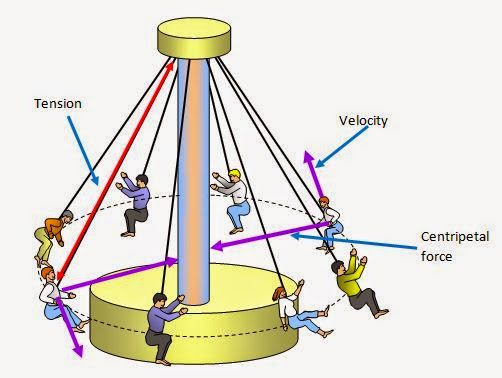
\includegraphics[width=0.7\textwidth]{img/constructivism_circular_motion.png}
		\caption{Real world example of circular motion\footfullcite{arulselvam2014}.}
		\label{fig:constructivism_example_part_1}
	\end{figure}
\end{frame}

\begin{frame}{Constructivism}
	\begin{figure}
		\centering
		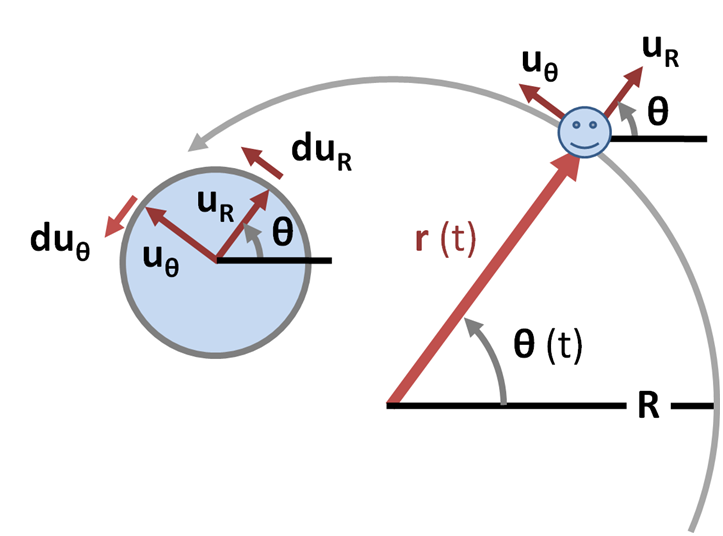
\includegraphics[width=0.7\textwidth]{img/constructivism_vectors.png}
		\caption{Abstracted example of circular motion\footfullcite{wikiUCM}.}
		\label{fig:constructivism_example_part_2}
	\end{figure}
\end{frame}

\begin{frame}{Problem Solving}
	\begin{enumerate}
		\item Expert vs. Novice Problem Solvers\footfullcite{maloney1994}
		\begin{itemize}
			\item Different Strategies\footfullcite{walsh2007}
			\item Epistemic Games\footfullcite{redish2006}
		\end{itemize}
		\item Polya's Method\footfullcite{polya1985}
		\begin{itemize}
			\item Define the Problem
			\item Create a Plan
			\item Solve the Problem
			\item Check Your Answer
		\end{itemize}
	\end{enumerate}
\end{frame}

\subsection{The CITA System}

\begin{frame}{Shallow CITA}
	\begin{figure}
		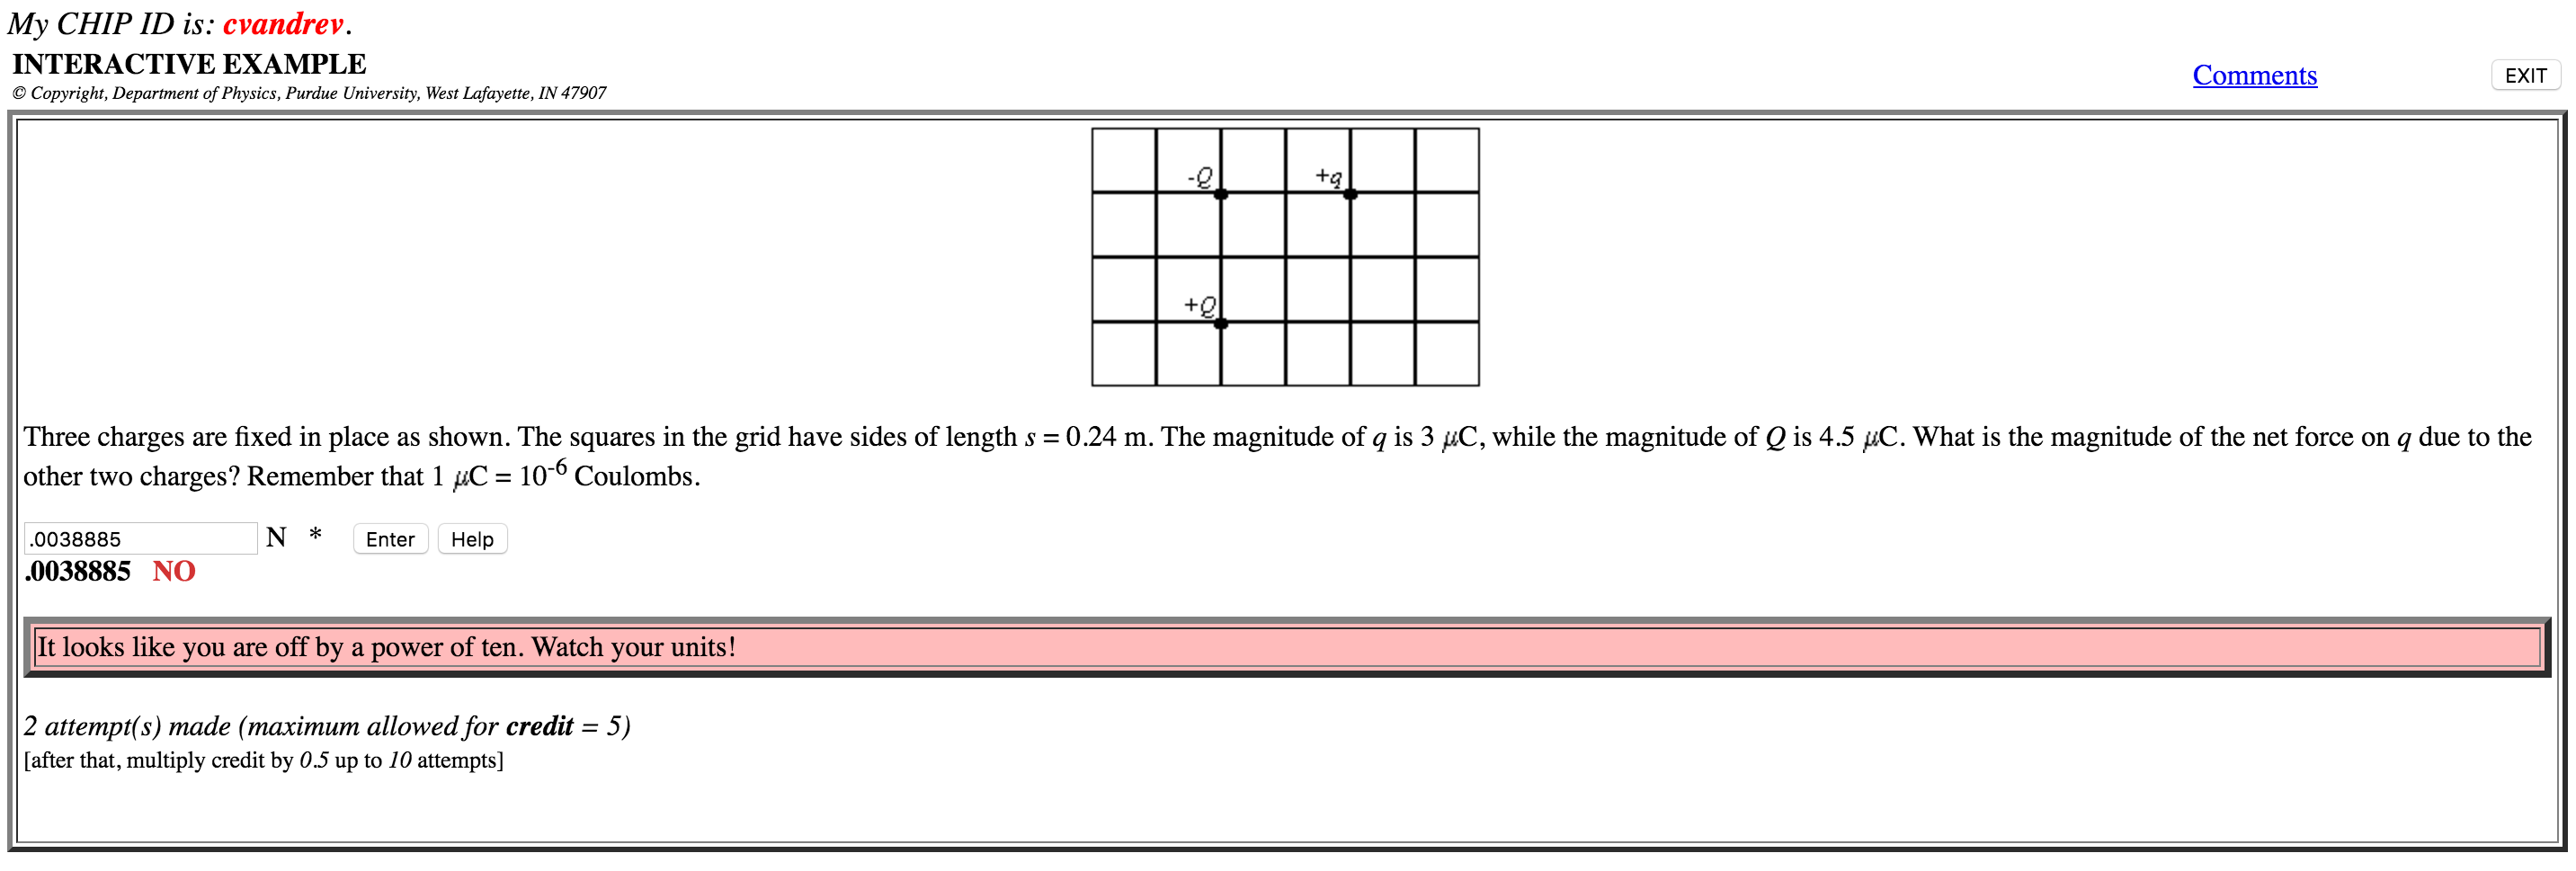
\includegraphics[width=1.0\textwidth]{img/shallow_cita_example.png}
		\caption{Shallow CITA is used to target specific errors that students make on their homework.}
		\label{fig:shallow_cita_example}
	\end{figure}
\end{frame}

\begin{frame}{Immersive CITA}
	\begin{figure}
		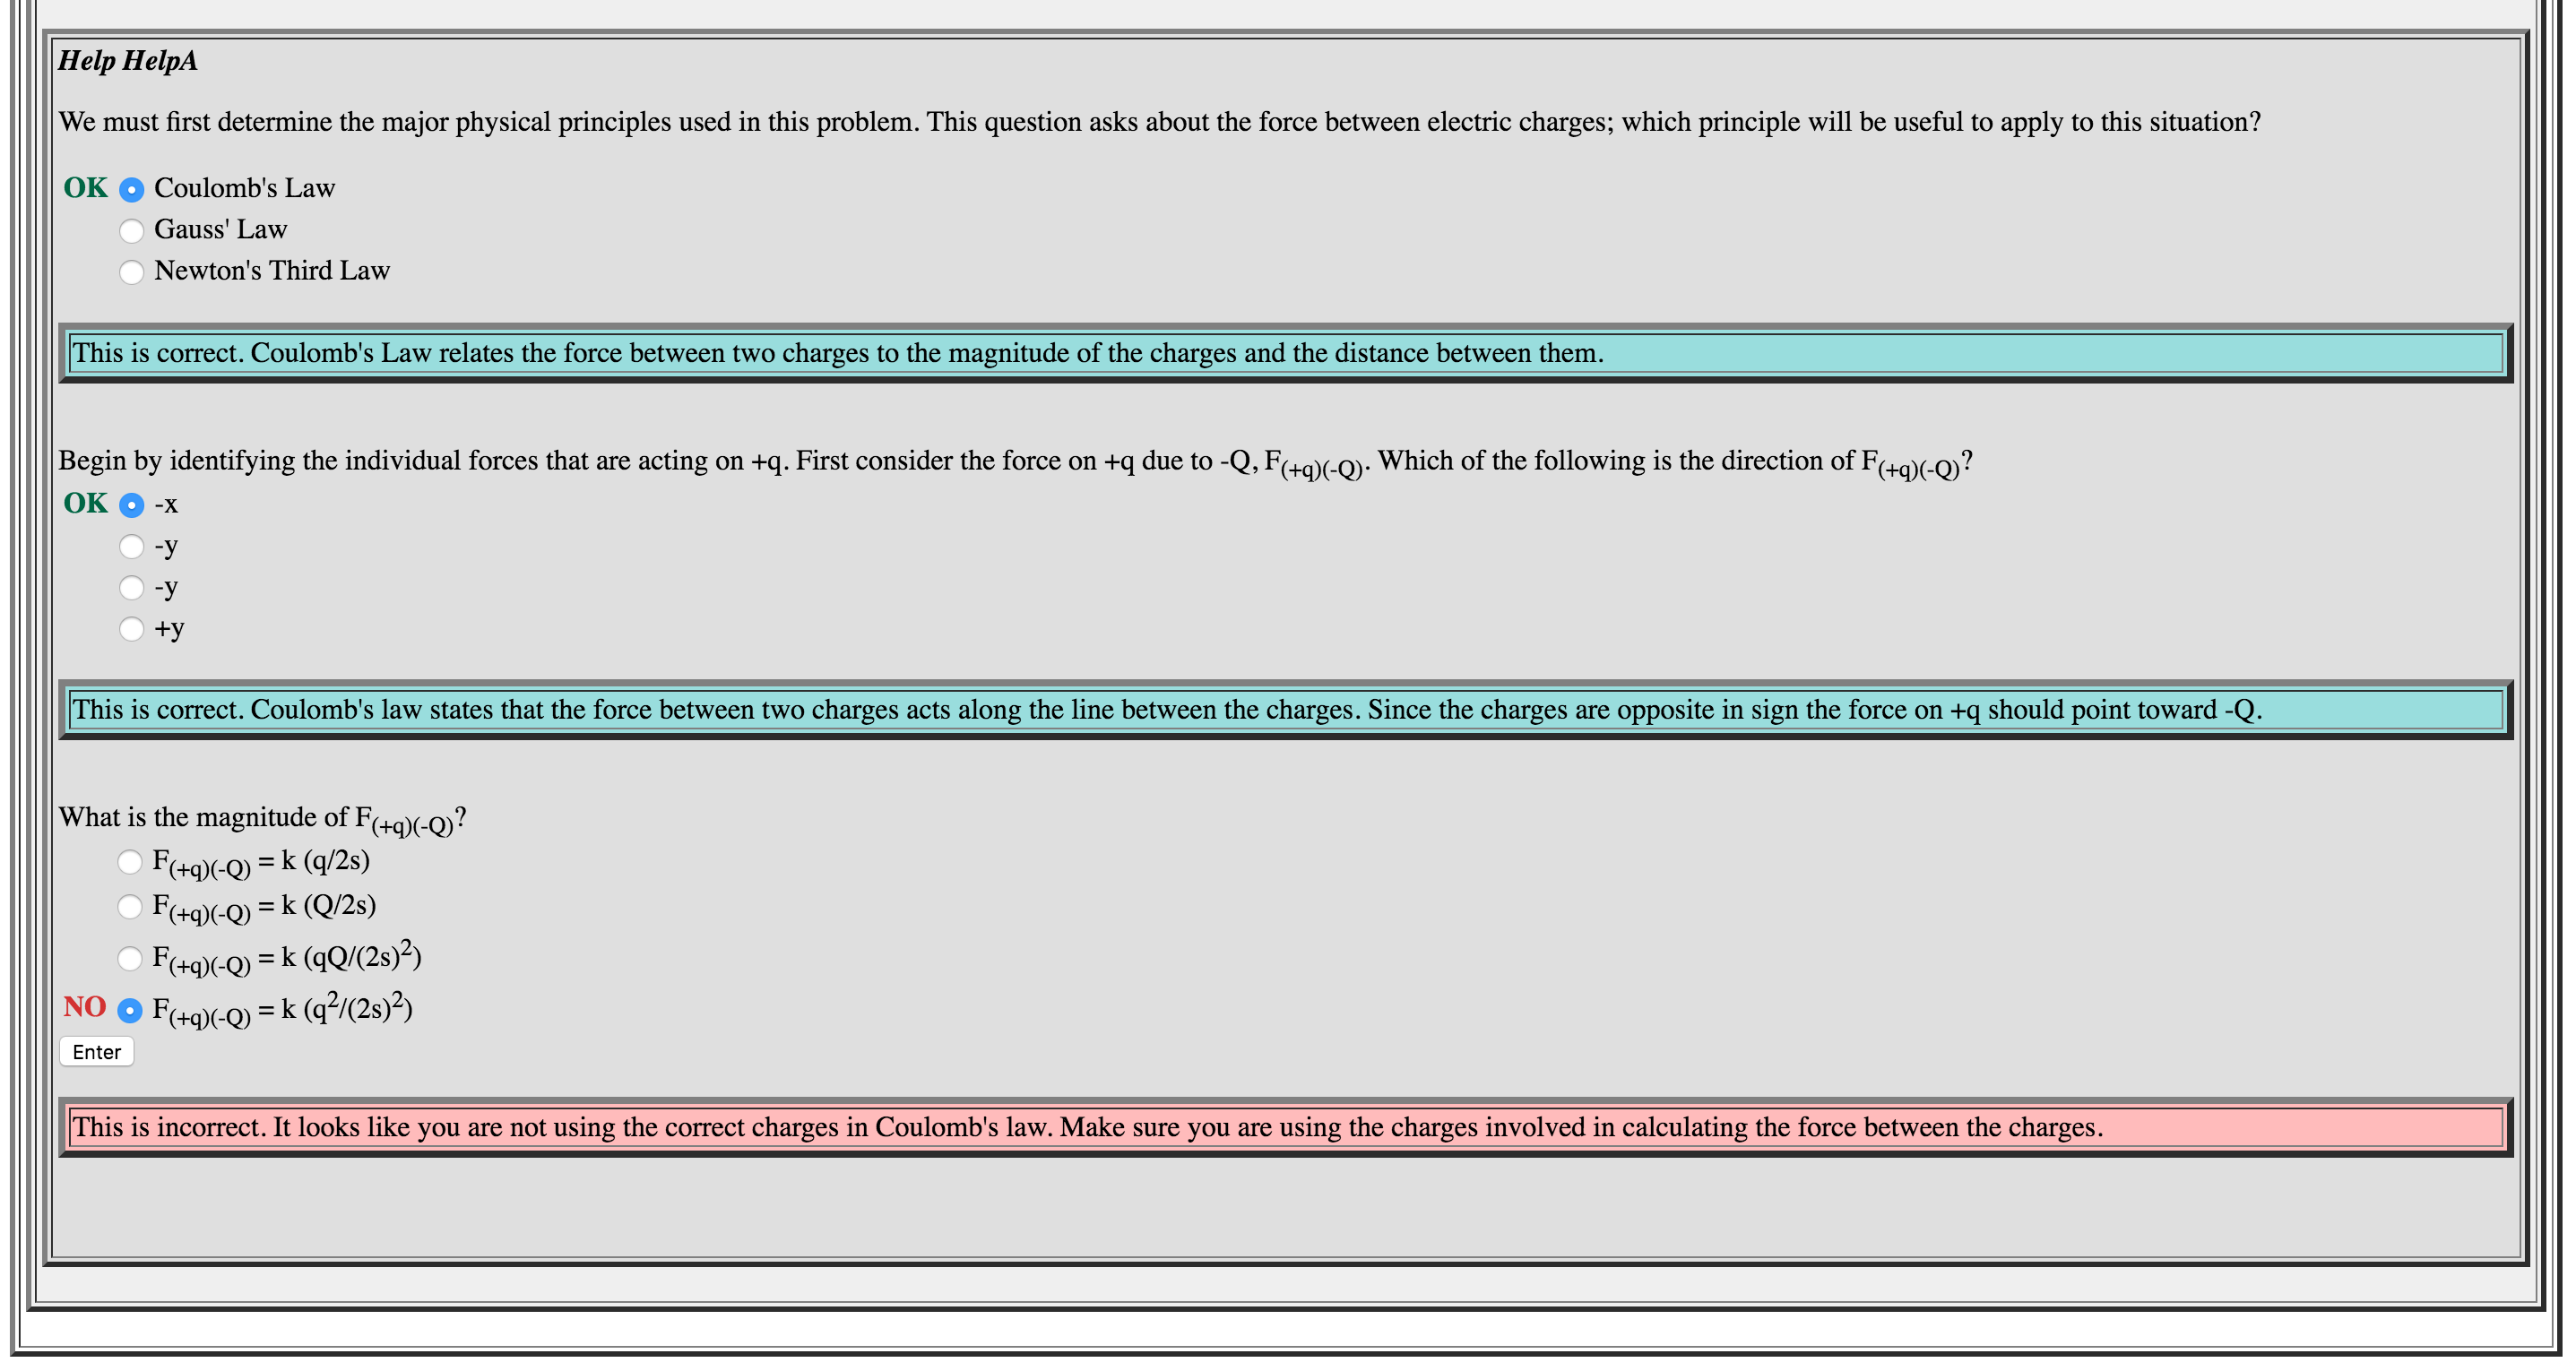
\includegraphics[width=1.0\textwidth]{img/immersive_cita_example.png}
		\caption{Immersive CITA provides a detailed tutorial that students can use to step through a problem.}
		\label{fig:immersive_cita_example}
	\end{figure}
\end{frame}

\begin{frame}{Immersive CITA}
	We implemented three different structures of tutorials.
	\vspace{5mm}
	\begin{enumerate}
		\item Detailed Step-by-Step Tutorial
		\vspace{3mm}
		\item Truncated Step-by-Step Tutorial
		\vspace{3mm}	
		\item Branching Tutorial
	\end{enumerate}
\end{frame}

\begin{frame}{Postscripts}
	\begin{figure}
		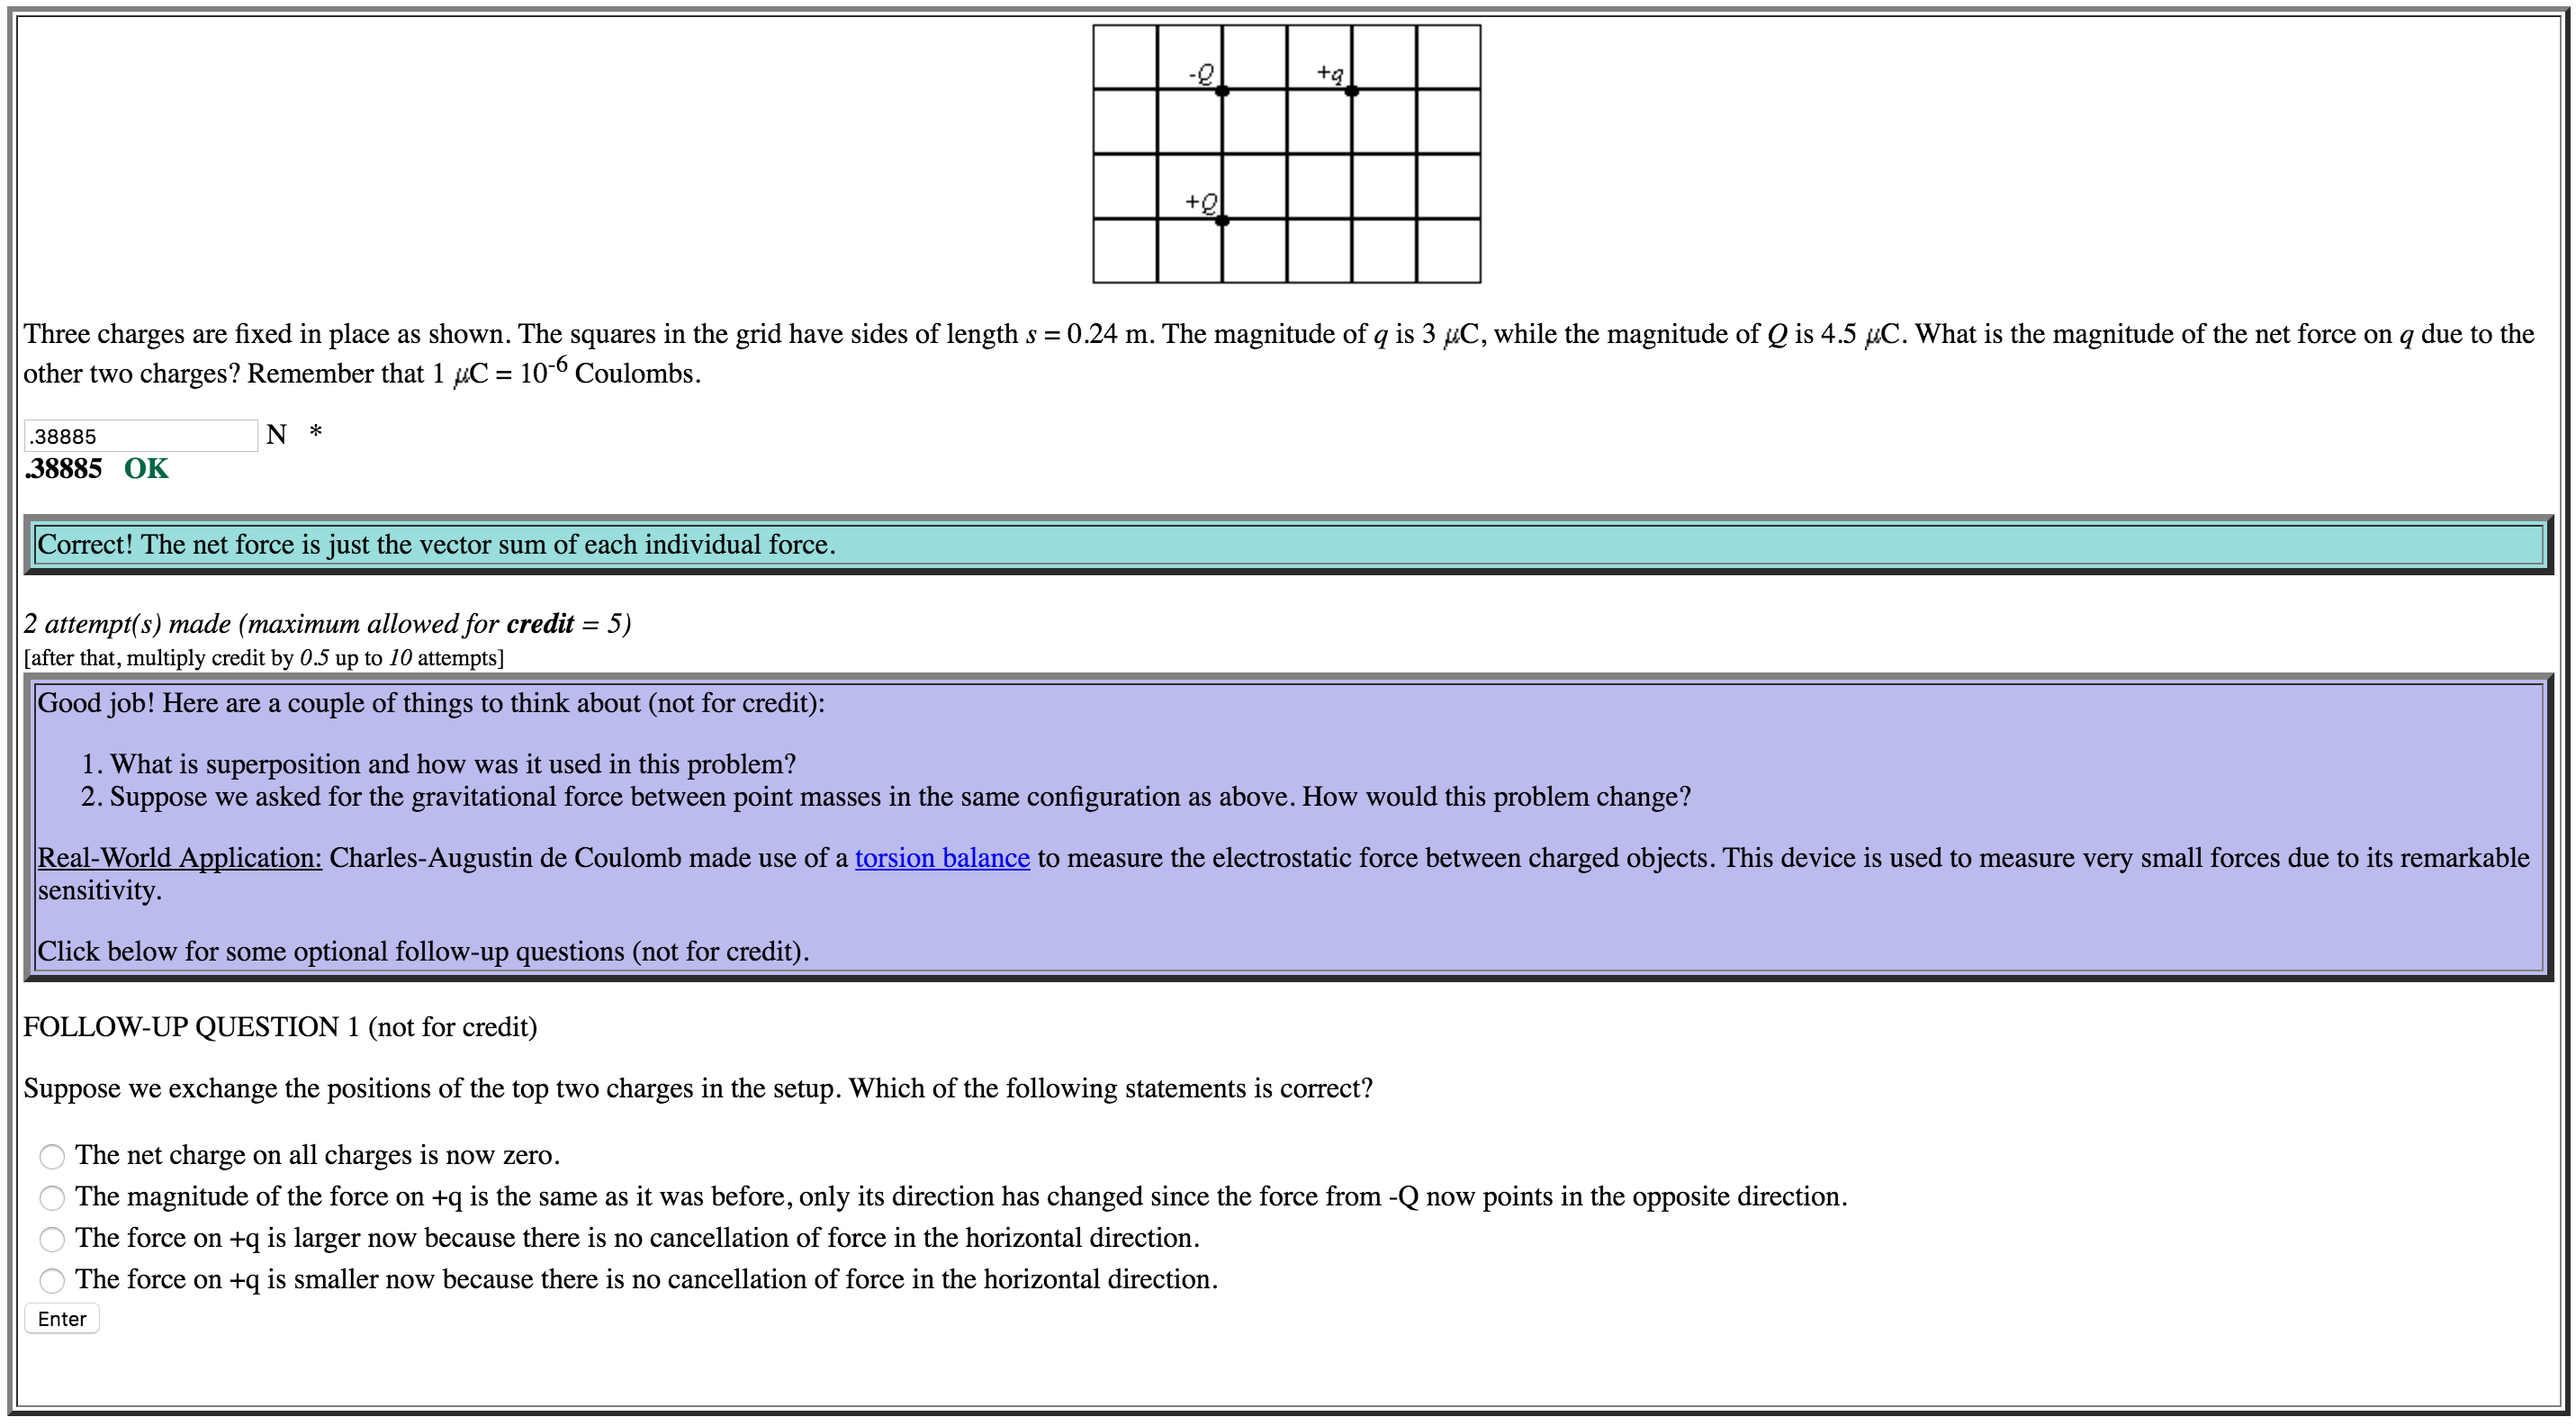
\includegraphics[width=1.0\textwidth]{img/postscript_example.png}
		\caption{Postscripts cover the last step of Polya's problem solving process.}
		\label{fig:postscript_example}
	\end{figure}
\end{frame}

\begin{frame}{Project Goals}
	\begin{enumerate}
		\item Design a framework that can be used to build online tutorials with multiple paths of analysis.
		\item Convert homework problems into interactive examples using Shallow CITA, Immersive CITA, and Postscripts.
		\item Analyze student performance between semesters and within a semester.
		\item Align teaching methods used in the classroom with those used on CITA.
	\end{enumerate}
\end{frame}

\begin{frame}{Research Questions}
	\begin{enumerate}
		\item How do the interactive examples influence the learning of physics concepts and problem solving skills?
		\vspace{5mm}
		\item Who is using the interactive examples on the homework?
		\vspace{5mm}
		\item What are students perceptions about the CITA system?
	\end{enumerate}
	\vspace{5mm}
	This presentation will focus mainly on \#1 with aspects of \#2 and \#3.
\end{frame}

%%%%%%%%%%%%%%%%%%%%%%%%%%%%%%%%%%%%%%%%%%%%%%%%%%%%%%
%%%%%%%%%%%%%%%%%%%%%%%%%%%%%%%%%%%%%%%%%%%%%%%%%%%%%%

\section{\scshape Methodology}

\subsection{Schedule of Development and Analysis}

\begin{frame}{Schedule of Development}
	\begin{table}[ht]
		\caption{In the spring semester of 2015 (and before), the CHIP homework system included 29 ``interactive examples'' that were originally developed by the faculty at UIUC (out of 139 homework problems total).}
		\begin{center}
			\begin{tabular}{|c|c|c|}
				\hline
				\textbf{Semester} & \textbf{Section} & \textbf{Version}\\
				\hline
				Spring 2015 and Before & Campus & Pre-CITA\\
				& Online & Pre-CITA\\
				\hline
				Summer 2015 & Online & 1.0 (Beta)\\
				\hline
				Fall 2015 & Campus & 2.0\\
				& Online & 1.0 (Beta)\\
				\hline
				Spring 2016 & Campus & 3.0\\
				& Online & 3.0\\
				\hline
				Summer 2016 & Online & 3.0\\
				\hline
			\end{tabular}
		\end{center}
		\label{tab:schedule}
	\end{table}
\end{frame}

\begin{frame}{Schedule of Analysis}
	We employed the sequential exploratory strategy since it is useful for the development and testing of a new instrument. One repeats phases of qualitative data analysis followed by phases of quantitative data analysis\footfullcite{creswell2003}.
	\vspace{3mm}
	\begin{enumerate}
		\item The project started with an analysis of student comments along with a literature review.
		\item We collected quantitative data during the semester and qualitative data at the end of the semester.
		\item We analyzed one type of data while collecting the other.
		\item We performed a final recap analysis in the summer of 2016.
	\end{enumerate}
\end{frame}

\subsection{Quantitative Procedures}

\begin{frame}{Quantitative Data}
	Quantitative data came from a variety of sources:
	\begin{itemize}
		\item Homework, Quiz, and Exam Scores
		\item BEMA Concept Inventory
		\item Multi-Step Problem
		\item End-of-Semester Surveys Based on Likert Scale
	\end{itemize}
\end{frame}

\begin{frame}{Quantitative Data}
	\begin{figure}
		\centering
		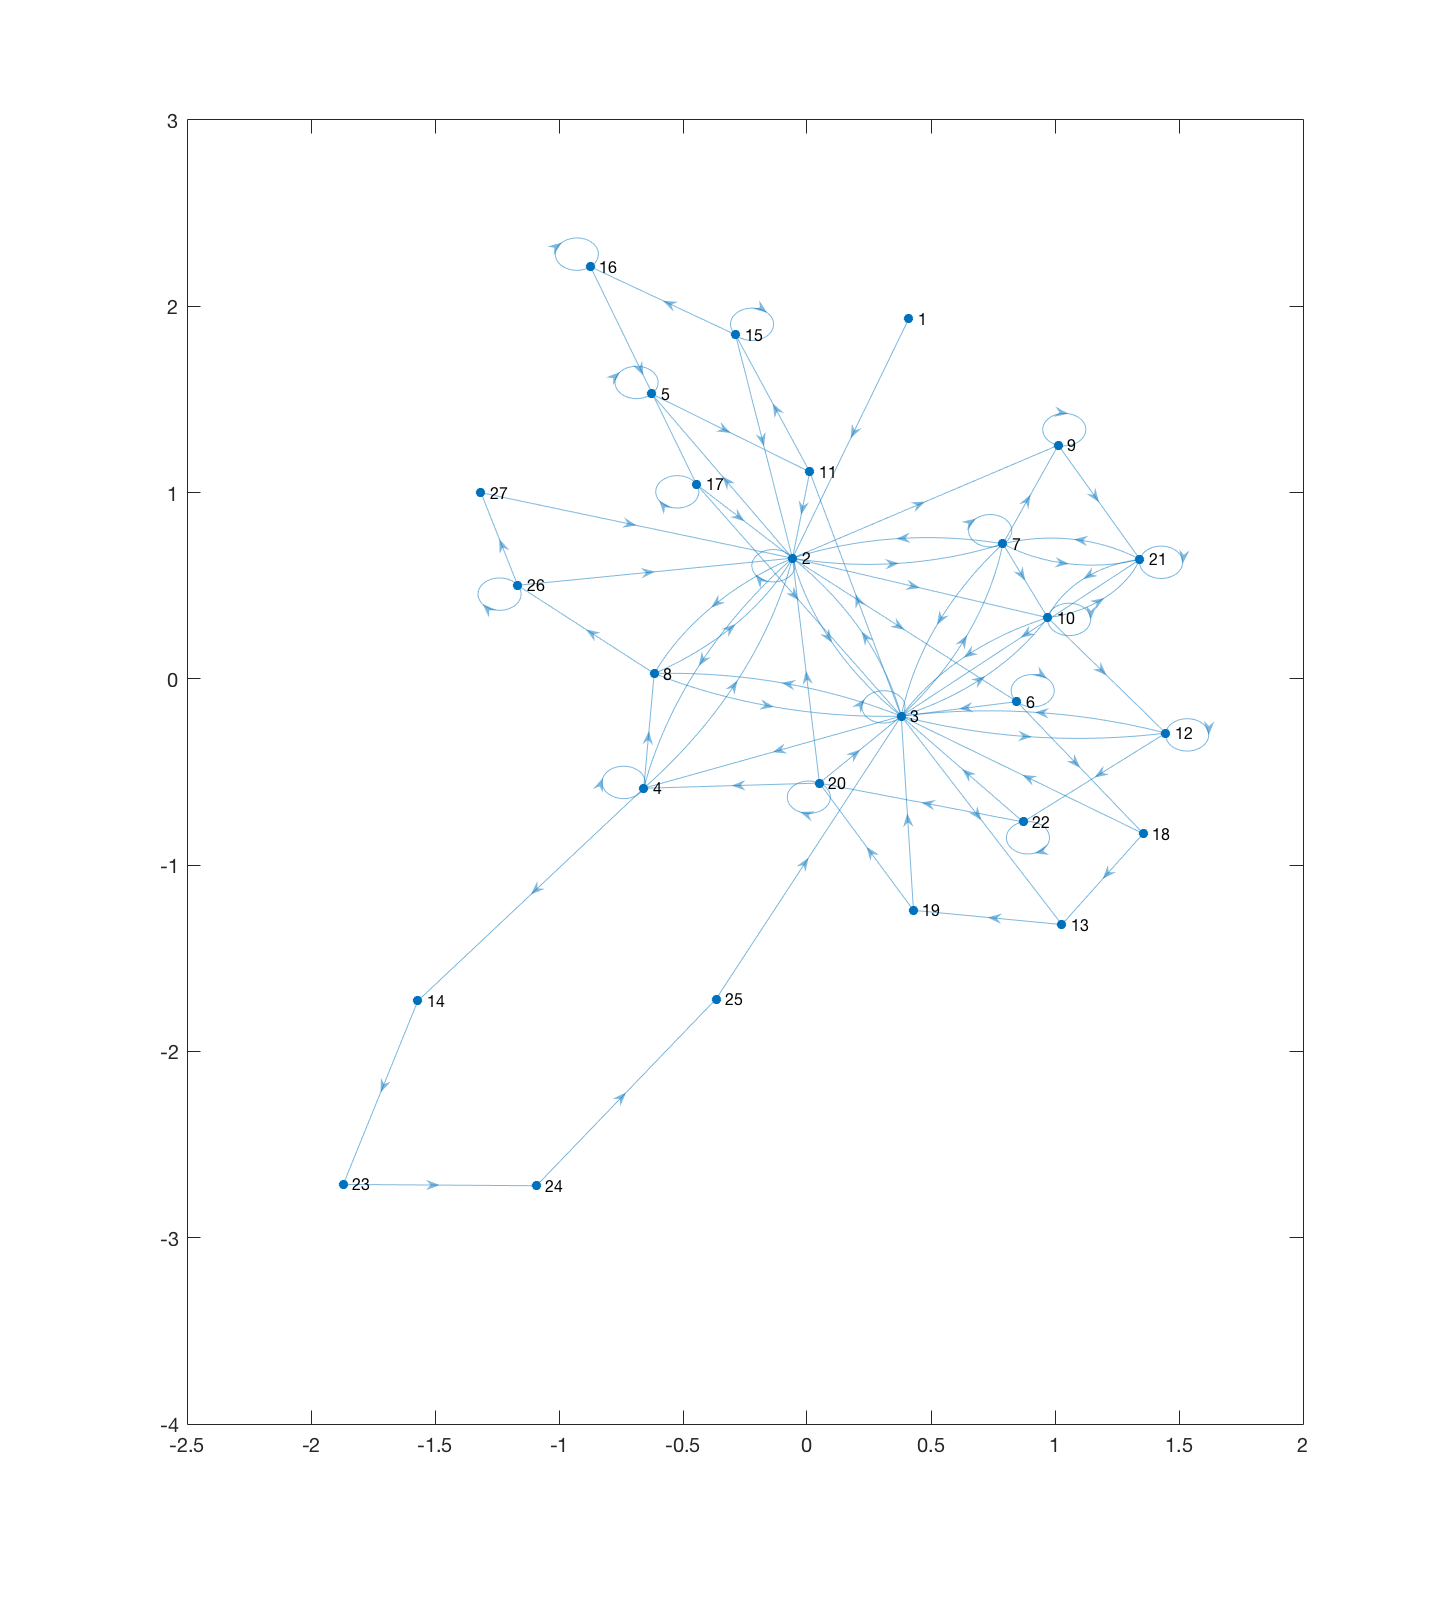
\includegraphics[width=0.35\textwidth]{img/matlab_example_1.png}
		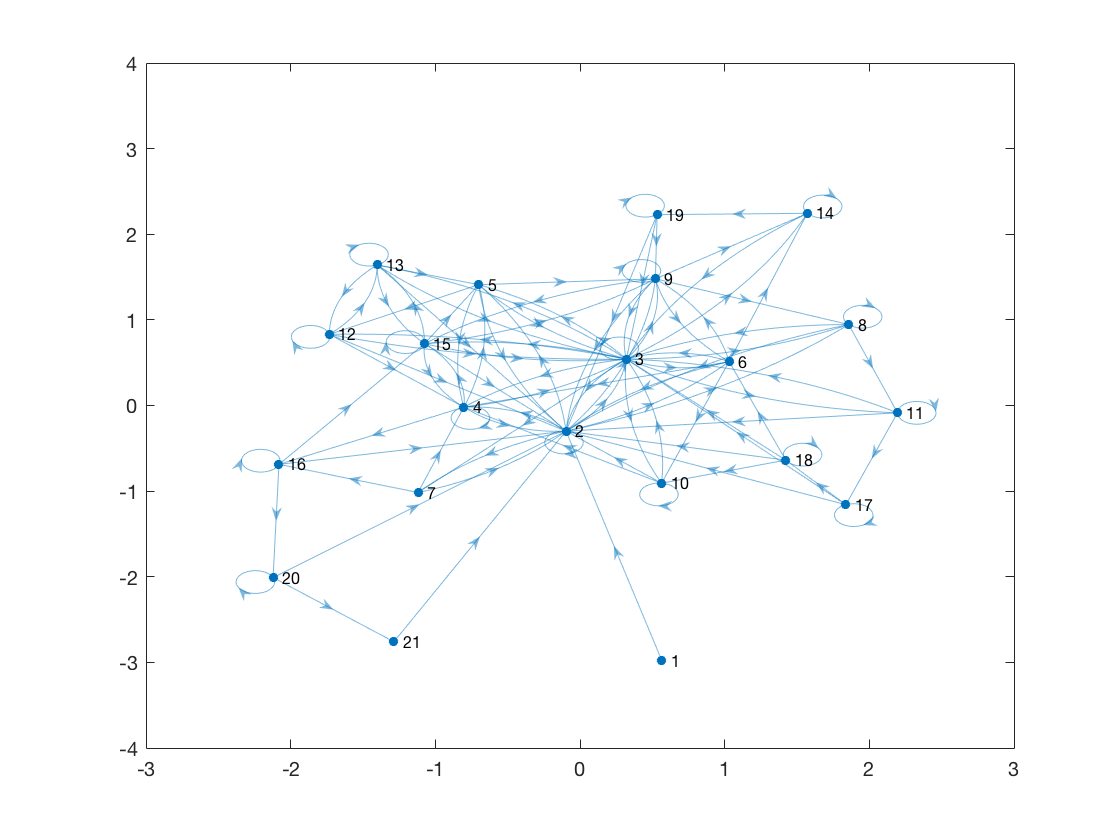
\includegraphics[width=0.50\textwidth]{img/matlab_example_2.png}
		\caption{We could track student clicks within the assignments.}
		\label{fig:matlab_examples}
	\end{figure}
\end{frame}

\subsection{Qualitative Procedures}

\begin{frame}{Strategy of Inquiry}
	Qualitative data for this project came from three major sources:
	\vspace{1mm}
	\begin{itemize}
		\item Final Question from Exit Survey
		\item Piazza Comments
		\item Focus Group Sessions
	\end{itemize}
	\vspace{5mm}
	We analyzed the qualitative data for this \textit{phenomenological study} using a three-cycle coding plan\footfullcite{saldana2012}:
	\vspace{1mm}
	\begin{itemize}
		\item \textbf{First Cycle:} Attribute and Descriptive Coding
		\item \textbf{Second Cycle:} Elaborative and Pattern Coding
		\item \textbf{Third Cycle:} Evaluation and Longitudinal Coding
	\end{itemize}
\end{frame}

\begin{frame}{Focus Group Sessions}
	Focus group sessions were used for a variety of reasons\footfullcite{hennink2014}:
	\vspace{1mm}
	\begin{itemize}
		\item Exploratory, explanatory, and evaluative research
		\item Large amounts of data with a range of viewpoints
		\item Limits researcher influence
	\end{itemize}
	\vspace{5mm}
	We used purposeful sampling as our design strategy\footfullcite{patton2015}:
	\vspace{1mm}
	\begin{itemize}
		\item Overall Impression of the Homework System
		\item Online vs. On-Campus Section of the Class
	\end{itemize}
\end{frame}

\begin{frame}{Roles of the Researchers}
	\begin{itemize}
		\item \textbf{Cyrus Vandrevala:} Teaching Assistant, Course Coordinator, Developed Online Course, Developed CITA Tutorials, Led Focus Group Sessions, Data Analysis
		\vspace{2mm}
		\item \textbf{Hisao Nakanishi:} Helped Develop CHIP and CITA, Scheduled Assignments, Answered Student Questions Through CHIP, Data Analysis
		\vspace{2mm}
		\item \textbf{Laura Pyrak-Nolte:} Course Administrator, Course Instructor, Lecturer for Online Sections, Data Analysis
		\vspace{2mm}
		\item \textbf{Lynn Bryan:} Theoretical Background
		\vspace{2mm}
		\item \textbf{Andrew Hirsch:} Instructor for PHYS 17200
		\vspace{2mm}
		\item \textbf{Gary Johns:} Teaching Assistant (24100 and 17200), Data Analysis
	\end{itemize}
\end{frame}

%%%%%%%%%%%%%%%%%%%%%%%%%%%%%%%%%%%%%%%%%%%%%%%%%%%%%%
%%%%%%%%%%%%%%%%%%%%%%%%%%%%%%%%%%%%%%%%%%%%%%%%%%%%%%

\section{\scshape Major Results}

\begin{frame}{I Have Picked Two Interesting Topics}
	There are a lot of interesting findings that have come from this study. We are going to focus on two.
	\vspace{3mm}
	\begin{enumerate}
		\item Gains in Student Performance
		\vspace{1mm}
		\item Student Desire for ``Efficiency''
	\end{enumerate}
\end{frame}

\subsection{Gains in Student Performance}

\begin{frame}{Overall Course Grade}
	\framesubtitle{Cut By PHYS 17200 Grade}
	\begin{columns}
		\begin{column}{0.5\textwidth}
			\begin{figure}
				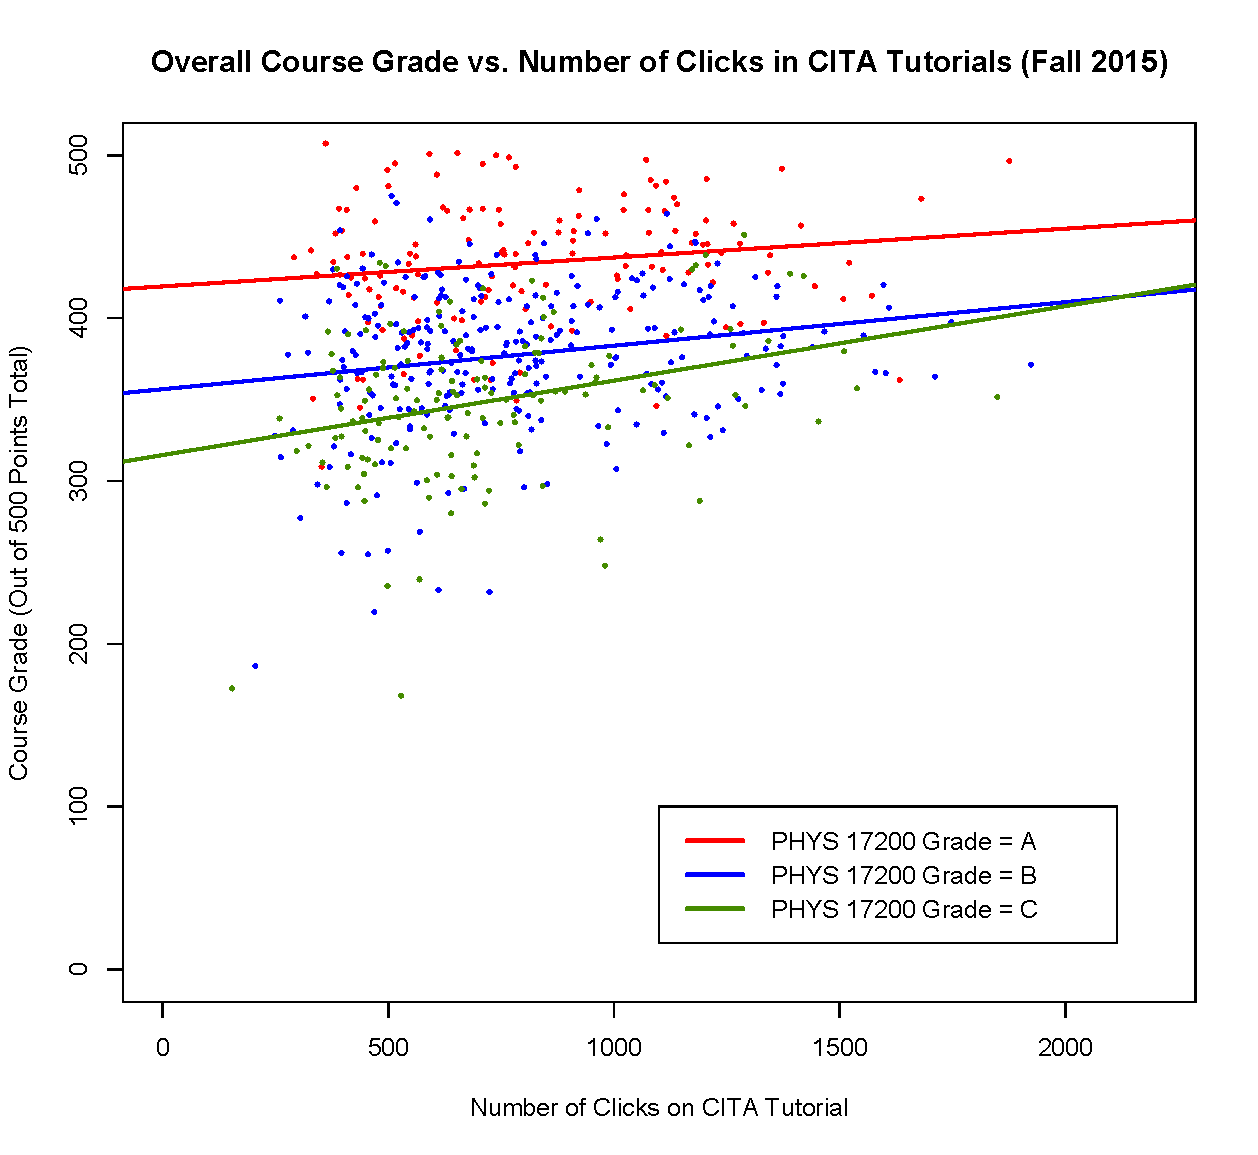
\includegraphics[width=1.0\textwidth]{img/overall_fa15_172.pdf}
			\end{figure}
		\end{column}
		\begin{column}{0.5\textwidth}	
			\begin{table}[ht]
				\begin{tabular}{|c|c|c|c|c|}
					\hline
					& \textbf{m} & \textbf{b} & \textbf{$R^2$} & \textbf{p}\\
					\hline
					A & 0.018 & 420 & 0.02 & 6.5e-2 \\
					B & 0.027 & 356 & 0.03 & 1.6e-3 \\
					C & 0.046 & 316 & 0.08 & 4.3e-4 \\
					\hline
				\end{tabular}
			\end{table}
		\end{column}
	\end{columns}
\end{frame}

\begin{frame}{Overall Course Grade}
	\framesubtitle{Cut By PHYS 17200 Grade}
	\begin{columns}
		\begin{column}{0.5\textwidth}
			\begin{figure}
				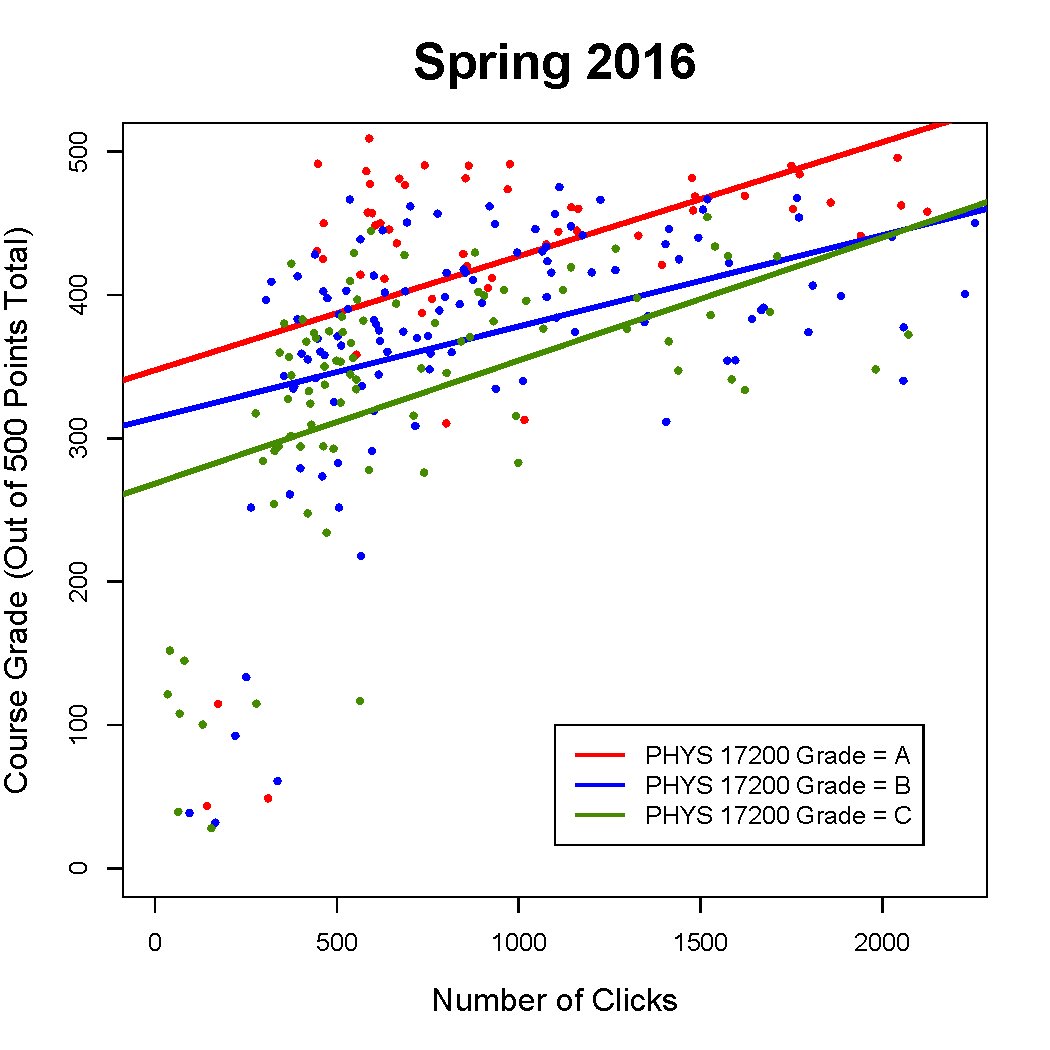
\includegraphics[width=1.0\textwidth]{img/overall_sp16_172.pdf}
			\end{figure}
		\end{column}
		\begin{column}{0.5\textwidth}	
			\begin{table}[ht]
				\begin{tabular}{|c|c|c|c|c|}
					\hline
					& \textbf{m} & \textbf{b} & \textbf{$R^2$} & \textbf{p}\\
					\hline
					A & 0.080 & 348 & 0.16 & 1.8e-3 \\
					B & 0.064 & 314 & 0.17 & 2.5e-6\\
					C & 0.086 & 268 & 0.24 & 7.8e-7 \\
					\hline
				\end{tabular}
			\end{table}
		\end{column}
	\end{columns}
\end{frame}

\begin{frame}{Overall Course Grade}
	\framesubtitle{Cut By PHYS 17200 Grade}
	\begin{figure}
		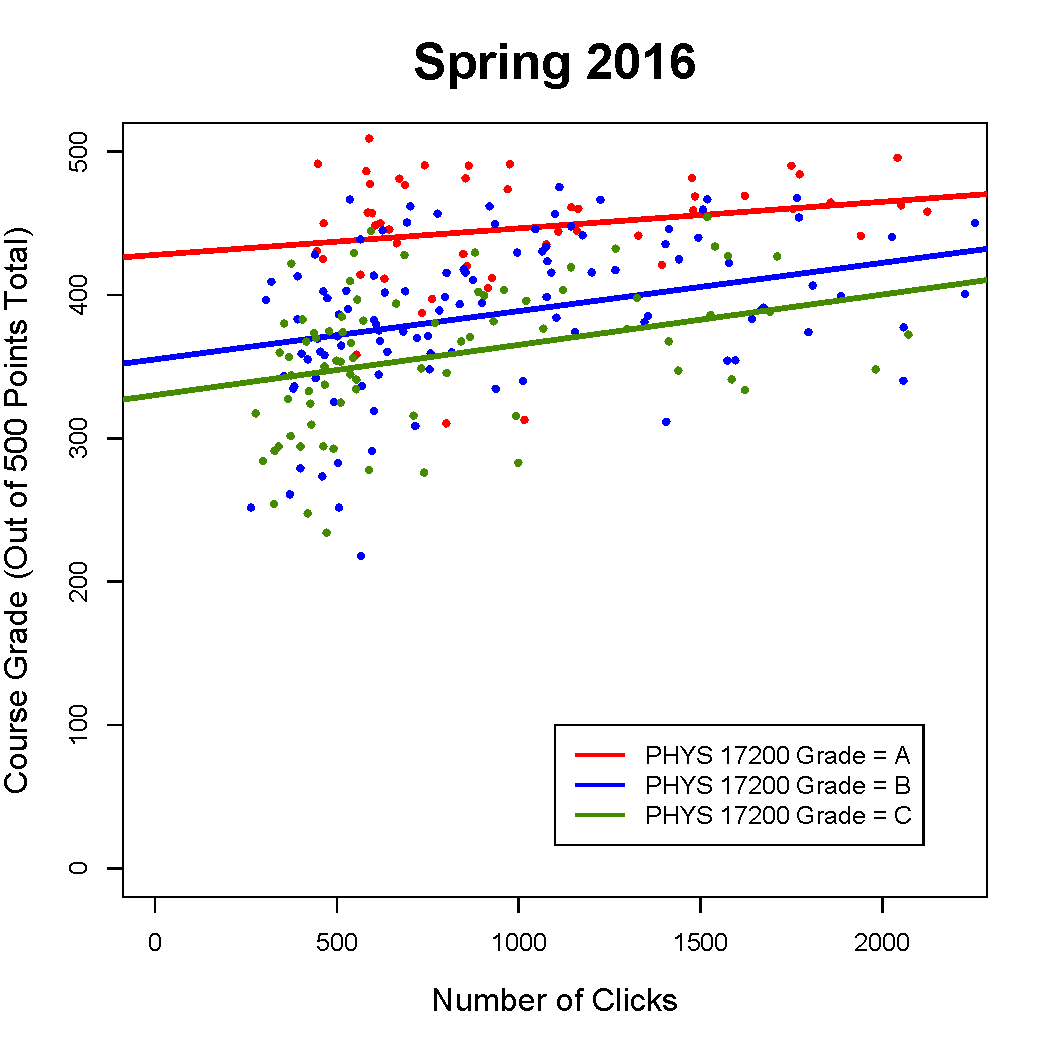
\includegraphics[width=0.5\textwidth]{img/overall_sp16_172_filtered.pdf}
	\end{figure}
	We still get statistically significant results for B and C grades if we eliminate the points in the lower-left hand corner of the graph. The slopes of the graphs drop by a factor of two or three.
\end{frame}

\begin{frame}{Overall Course Grade}
	\framesubtitle{Cut By Previous Calculus Grade}
	\begin{columns}
		\begin{column}{0.5\textwidth}
			\begin{figure}
				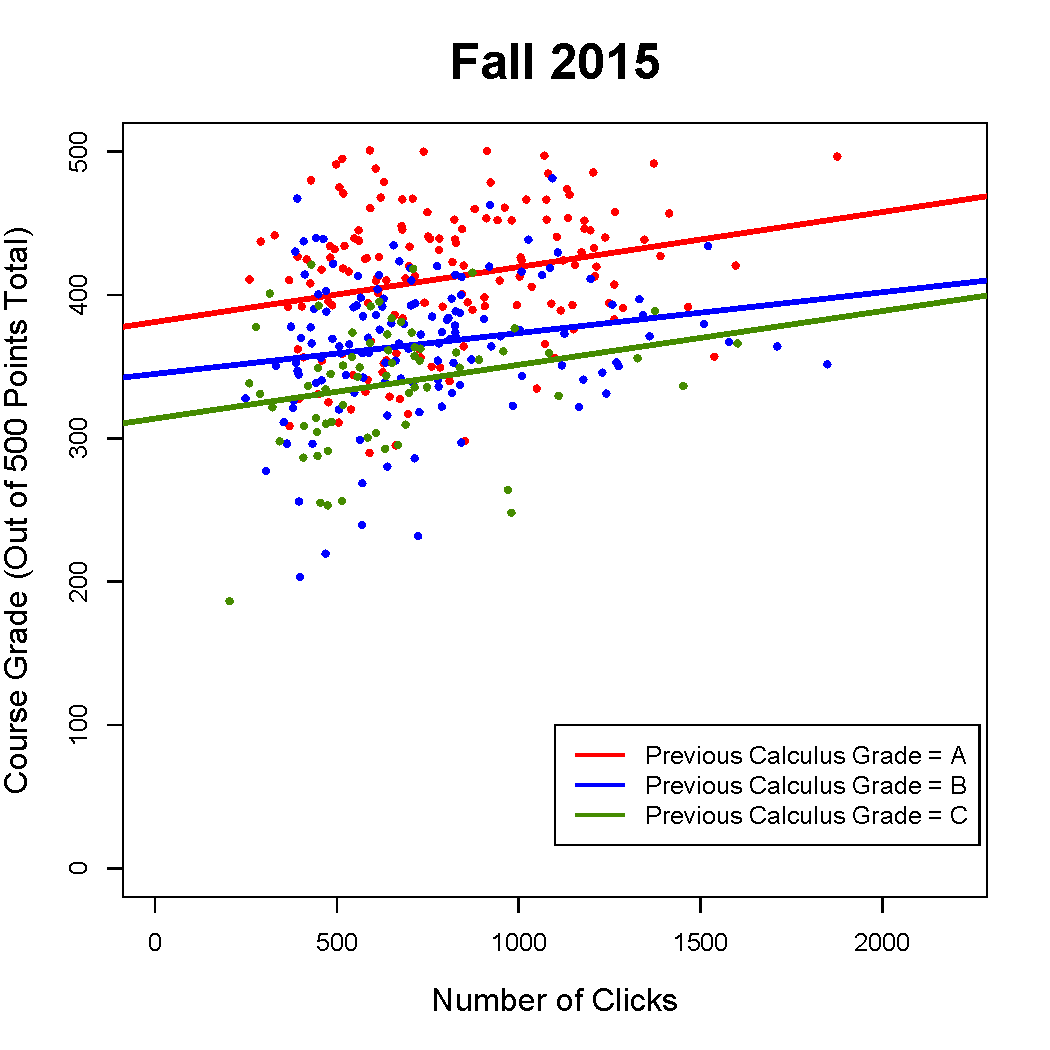
\includegraphics[width=1.0\textwidth]{img/overall_fa15_calculus.pdf}
			\end{figure}
		\end{column}
		\begin{column}{0.5\textwidth}	
			\begin{table}[ht]
				\begin{tabular}{|c|c|c|c|c|}
					\hline
					& \textbf{m} & \textbf{b} & \textbf{$R^2$} & \textbf{p}\\
					\hline
					A & 0.038 & 381 & 0.05 & 3.1e-3 \\
					B & 0.028 & 345 & 0.03 & 3.2e-2\\
					C & 0.038 & 314 & 0.04 & 5.3e-2 \\
					\hline
				\end{tabular}
			\end{table}
		\end{column}
	\end{columns}
\end{frame}

\begin{frame}{Overall Course Grade}
	\framesubtitle{Cut By Previous Calculus Grade}
	\begin{columns}
		\begin{column}{0.5\textwidth}
			\begin{figure}
				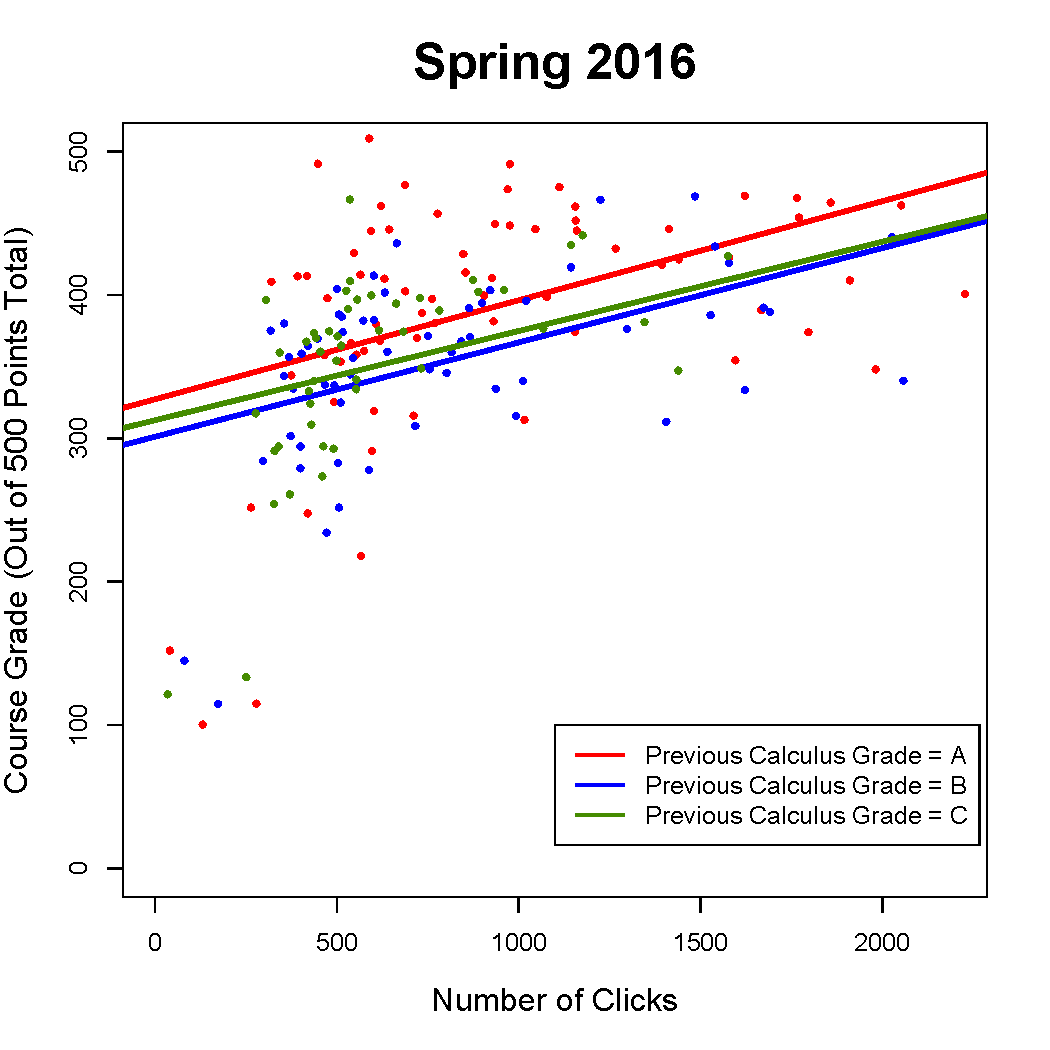
\includegraphics[width=1.0\textwidth]{img/overall_sp16_calculus.pdf}
			\end{figure}
		\end{column}
		\begin{column}{0.5\textwidth}	
			\begin{table}[ht]
				\begin{tabular}{|c|c|c|c|c|}
					\hline
					& \textbf{m} & \textbf{b} & \textbf{$R^2$} & \textbf{p}\\
					\hline
					A & 0.069 & 327 & 0.17 & 2.1e-4 \\
					B & 0.066 & 301 & 0.22 & 1.0e-4\\
					C & 0.062 & 313 & 0.17 & 1.9e-3 \\
					\hline
				\end{tabular}
			\end{table}
		\end{column}
	\end{columns}
\end{frame}

\begin{frame}{Overall Course Grade}
	\framesubtitle{Cut By Section}
	\begin{columns}
		\begin{column}{0.5\textwidth}
			\begin{figure}
				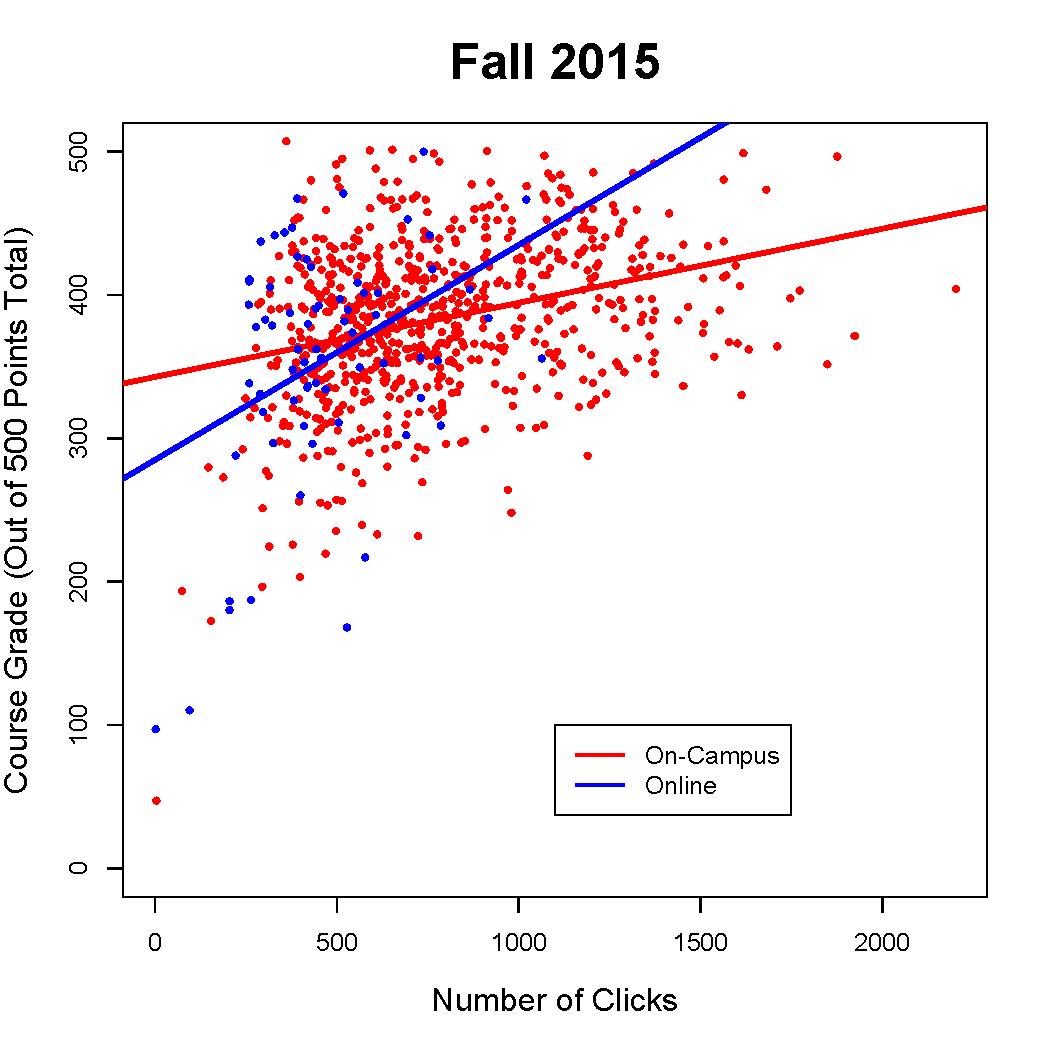
\includegraphics[width=1.0\textwidth]{img/overall_fa15_section.pdf}
			\end{figure}
		\end{column}
		\begin{column}{0.5\textwidth}	
			\begin{table}[ht]
				\begin{tabular}{|c|c|c|c|c|}
					\hline
					& \textbf{m} & \textbf{b} & \textbf{$R^2$} & \textbf{p}\\
					\hline
					C & 0.052 & 343 & 0.10 & 2.2e-16 \\
					O & 0.150 & 285 & 0.13 & 1.3e-3\\
					\hline
				\end{tabular}
			\end{table}
			On-Campus = C\\
			Online = O
		\end{column}
	\end{columns}
\end{frame}

\begin{frame}{Overall Course Grade}
	\framesubtitle{Cut By Section}
	\begin{columns}
		\begin{column}{0.5\textwidth}
			\begin{figure}
				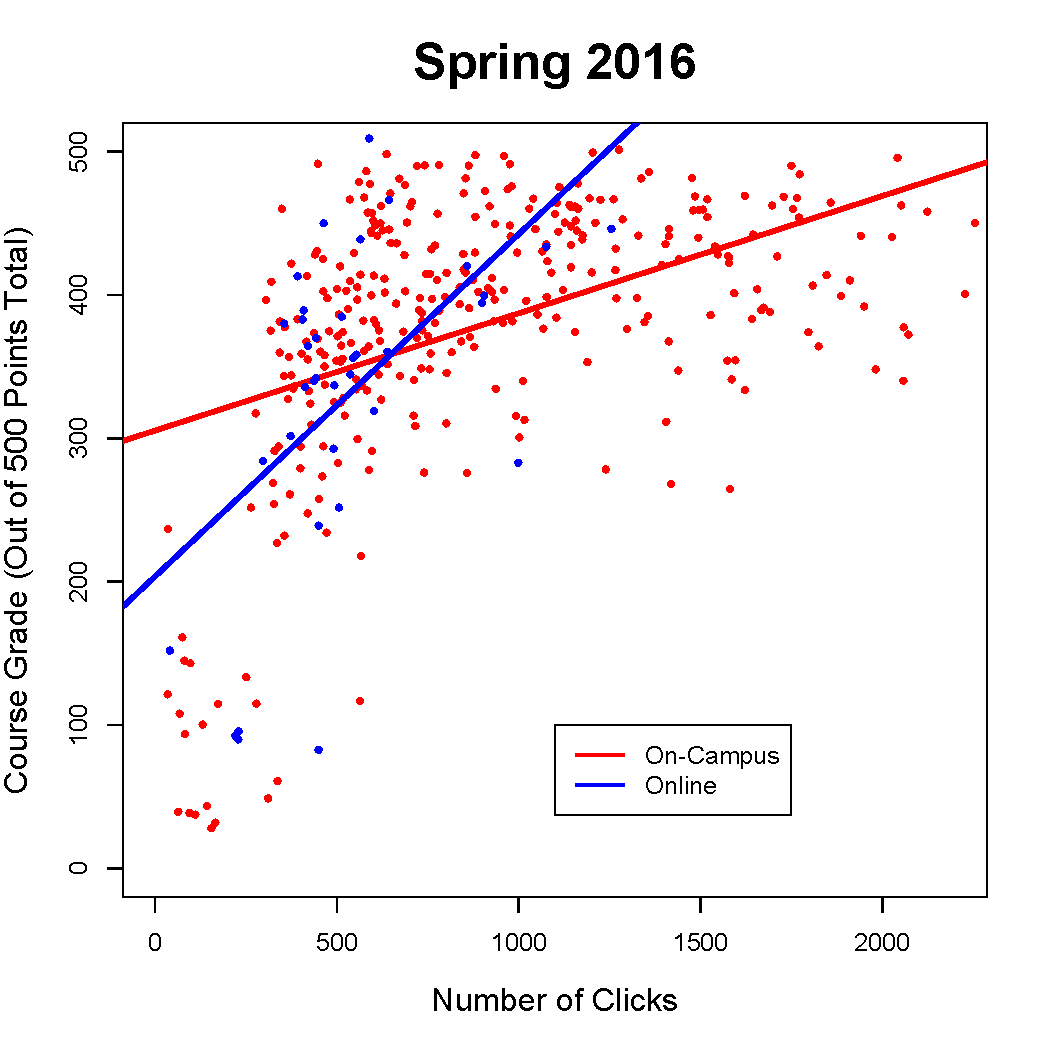
\includegraphics[width=1.0\textwidth]{img/overall_sp16_section.pdf}
			\end{figure}
		\end{column}
		\begin{column}{0.5\textwidth}	
			\begin{table}[ht]
				\begin{tabular}{|c|c|c|c|c|}
					\hline
					& \textbf{m} & \textbf{b} & \textbf{$R^2$} & \textbf{p}\\
					\hline
					C & 0.080 & 305 & 0.20 & 2.2e-16 \\
					O & 0.239 & 204 & 0.28 & 6.0e-4\\
					\hline
				\end{tabular}
			\end{table}
			On-Campus = C\\
			Online = O
		\end{column}
	\end{columns}
\end{frame}

\begin{frame}{Overall Course Grade}
	\begin{enumerate}
		\item The linear fit is getting better with each passing semester.
		\vspace{2mm}
		\item These small slopes add up to big gains in the class.
		\vspace{2mm}
		\item Online students are clicking far less than on-campus students (skewing the linear models).
	\end{enumerate}
\end{frame}

\begin{frame}{BEMA Normalized Gain}
	\begin{figure}[ht]
		\centering
		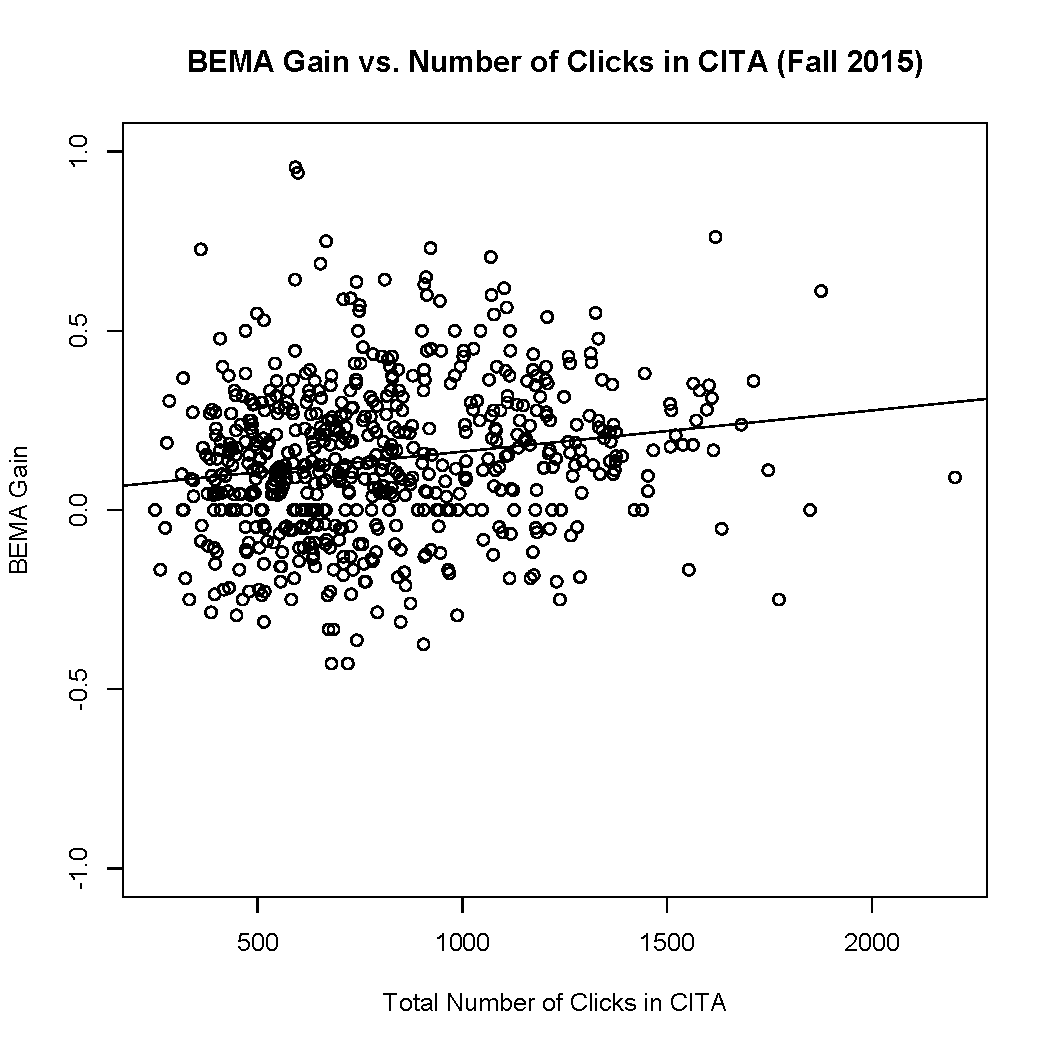
\includegraphics[width=0.45\textwidth]{img/bema_fa15_gain.pdf}
		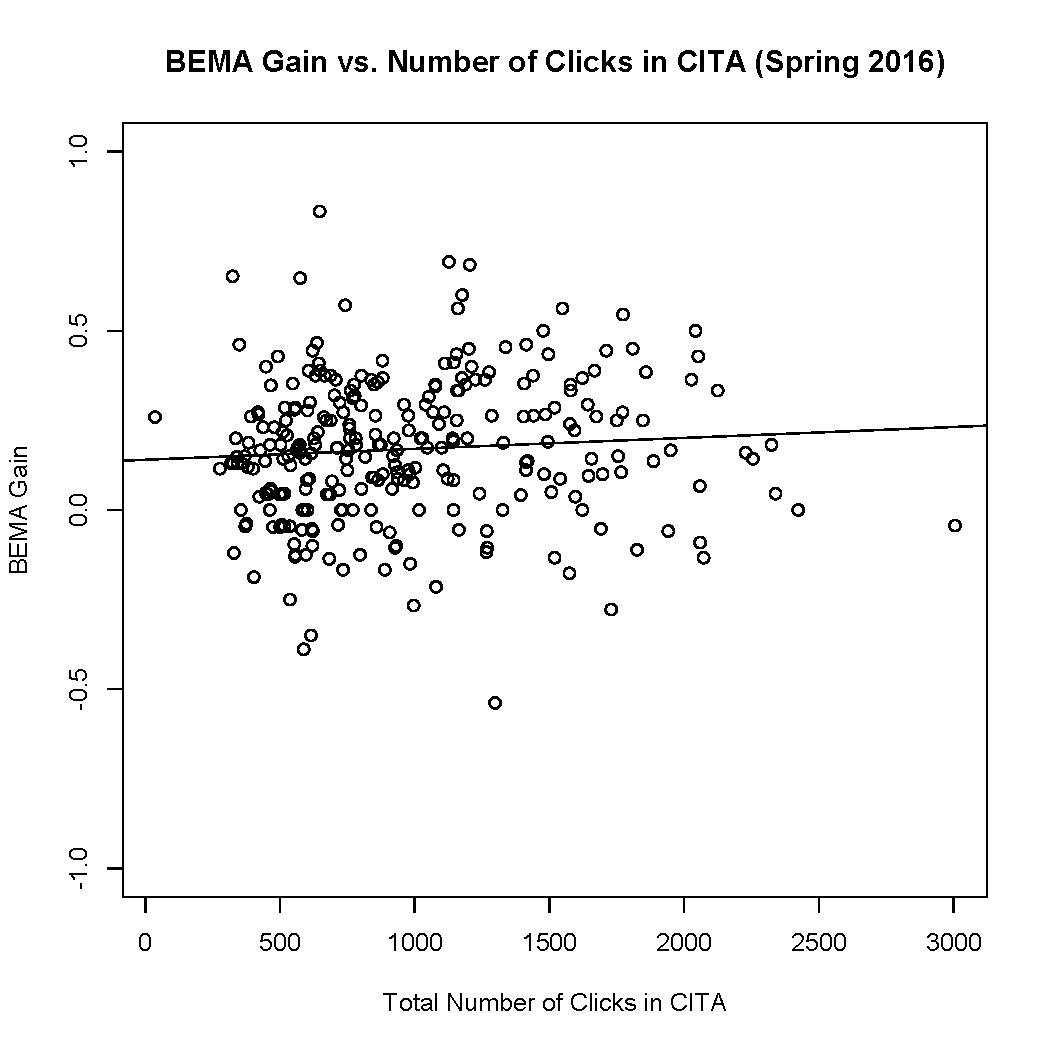
\includegraphics[width=0.45\textwidth]{img/bema_sp16_gain.pdf}
		\caption{Student gains on the BEMA as a function of number of CITA clicks. The students shown in these plots are all in on-campus sections of PHYS 24100. The spring semester has a p-value of 0.2025 and an $R^2$ value of 0.00. The fall semester has a p-value of 1.48e-5 and an $R^2$ value of 0.03.}
	\end{figure}
\end{frame}

\begin{frame}{Multi-Step Problem}
	\begin{itemize}
		\item We administered an optics problem in the on-campus recitations under test-like conditions as a measure of student problem solving abilities.
		\item We then developed a six point rubric to assess student performance during each semester.
	\end{itemize}
	\vspace{1mm}
	\noindent\makebox[\linewidth]{\rule{12cm}{0.4pt}}
	
	{\small A laser beam of power P = 10.0 W and diameter D = 1.00 mm is directed upward onto one circular face of a perfectly reflecting cylinder. The cylinder levitates due to the balance between the upward radiation force and the downward gravitational force. If the density of the cylinder is 1.25 g/cm3, and the diameter of the circular face is 0.50 mm, what is the height H of the cylinder?}
\end{frame}

\begin{frame}{Multi-Step Problem}
\begin{table}[ht]
  \caption{A chi-squared test of the data above yields a p-value of 0.001 and an effect size (Cramer's V) of 0.117. We are seeing improvements in student's scores between spring 2015 and spring 2016.}
  \begin{center}
    \begin{tabular}{|c|c|c|c|}
      \hline
      \textbf{Score} & \textbf{Spring 2015} & \textbf{Fall 2015} & \textbf{Spring 2016}\\
      \hline
      {\color{DeepPink4} 0} &  {\color{DeepPink4} 11.32\%} &  {\color{DeepPink4} 9.05\%} &  {\color{DeepPink4} 8.08\%}\\
      \hline
      1 & 8.63\% & 7.78\% & 8.58\%\\
      \hline
      {\color{DeepPink4} 2} & {\color{DeepPink4} 19.68\%} & {\color{DeepPink4} 14.92\%} & {\color{DeepPink4} 7.58\%}\\
      \hline
      3 & 33.96\% & 31.75\% & 35.86\%\\
      \hline
      {\color{DodgerBlue3} 4} & {\color{DodgerBlue3} 19.68\%} & {\color{DodgerBlue3} 27.14\%} & {\color{DodgerBlue3} 26.77\%}\\
      \hline
      {\color{DodgerBlue3} 5} & {\color{DodgerBlue3} 6.20\%} & {\color{DodgerBlue3} 7.46\%} & {\color{DodgerBlue3} 8.58\%}\\
      \hline
      {\color{DodgerBlue3} 6} & {\color{DodgerBlue3} 0.53\%} & {\color{DodgerBlue3} 1.90\%} & {\color{DodgerBlue3} 4.55\%}\\
      \hline
      \textbf{Mean} & \textbf{2.63} & \textbf{2.90} & \textbf{2.95}\\
      \hline
      \textbf{Standard Deviation} & \textbf{1.39} & \textbf{1.42} & \textbf{1.36}\\
      \hline
    \end{tabular}
  \end{center}
  \label{tab:multi-step}
\end{table}
\end{frame}

\begin{frame}{Multi-Step Problem}
	\begin{figure}
		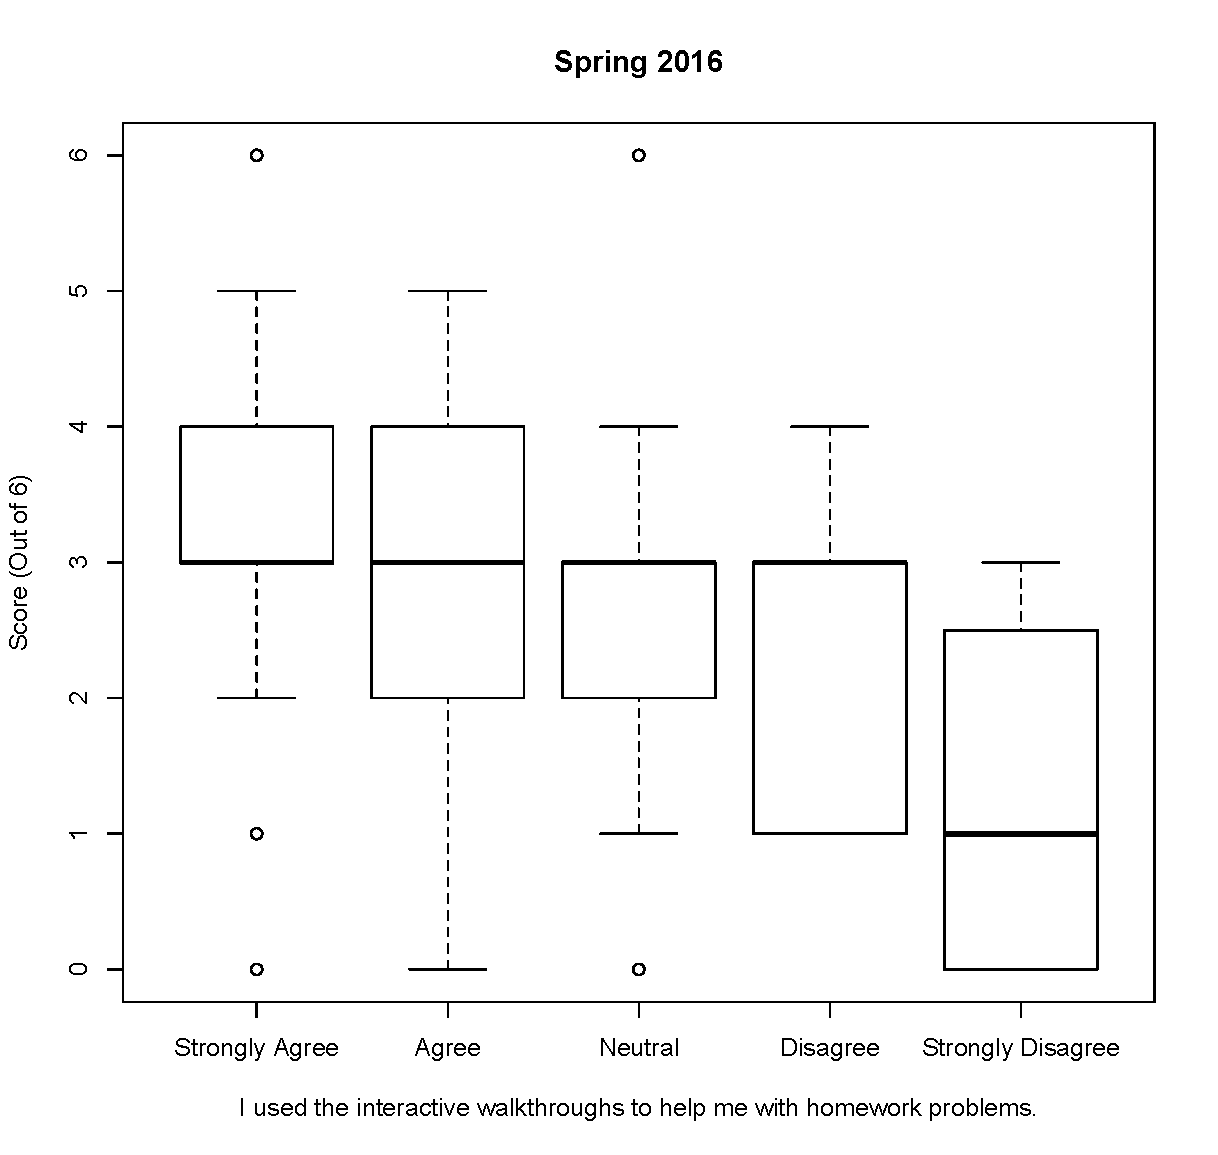
\includegraphics[width=0.7\textwidth]{img/multi-step_vs_reported_use.pdf}
	\end{figure}
\end{frame}

\subsection{``Efficiency'' and Learning}

\begin{frame}
	\begin{center}
		{\large Switching now to a discussion of student's desire for efficiency.}
	\end{center}
\end{frame}

\begin{frame}{Efficiency}
	\begin{itemize}
		\item This was the part of the research that I found most interesting because it was a bit unexpected.
		\item Students really liked the fact that our tutorials were optional and that they could choose when to enter and exit.
		\item More than anything else, students are interested in completing the homework as quickly and efficiently as possible.
	\end{itemize}
\end{frame}

\begin{frame}{Efficiency}
	\begin{quote}
		There's, every once in a while I have to go through, do something [an Immersive CITA tutorial] twice, but usually it's only once.
	\end{quote}
	\vspace{5mm}
	- Student, Spring 2016
\end{frame}

\begin{frame}{Efficiency}
	\begin{quote}
		So, typically, um, I usually start, I'd say I probably work about 10:00 to noon on Friday mornings,...
	\end{quote}
	\vspace{5mm}
	- Student, Spring 2016
\end{frame}

\begin{frame}{Efficiency}
	\begin{quote}
		Um, unfortunately sometimes I'm in a haste to get the homework done so I don't always have time to you know, read them [the Postscripts]. I'm just like, ``Okay, next problem.''
	\end{quote}
	\vspace{5mm}
	- Student, Spring 2016
\end{frame}

\begin{frame}{Efficiency}
	\begin{itemize}
		\item Students create a ``toolbox'' of resources that they use to complete the homework problems.
		\item Back in the old days there were fewer resources available, and it was sometimes difficult to switch between sources. The internet allows students to switch between sources at a moment's notice.
		\item Students switch resources when the perceived benefit of a resource is less than the cost needed to continue using it.
	\end{itemize}
\end{frame}

\begin{frame}{Efficiency}
	\begin{quote}
		Uhm, I mainly use my notes to help me, the ones that I take in lecture. And then go to online, and then the book. I'm... actually not sure where my book is right now. But, uhm, yeah it's not really... Mostly notes and then a little bit online.
	\end{quote}
	\vspace{5mm}
	- Student, Fall 2015
\end{frame}

\begin{frame}{Efficiency}
	\framesubtitle{End of Problem}
	\begin{figure}
		\centering
		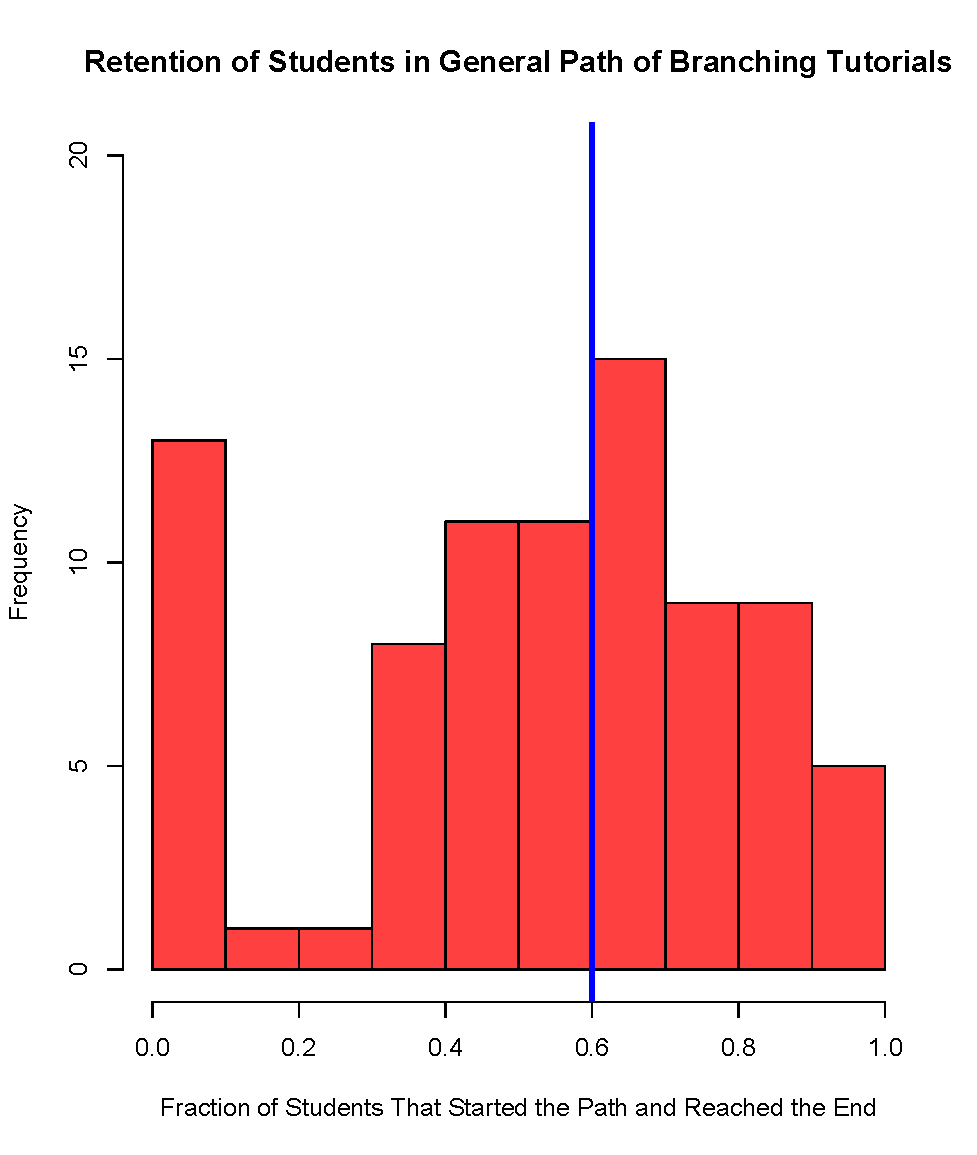
\includegraphics[width=0.46\textwidth]{img/retention_general.pdf}
		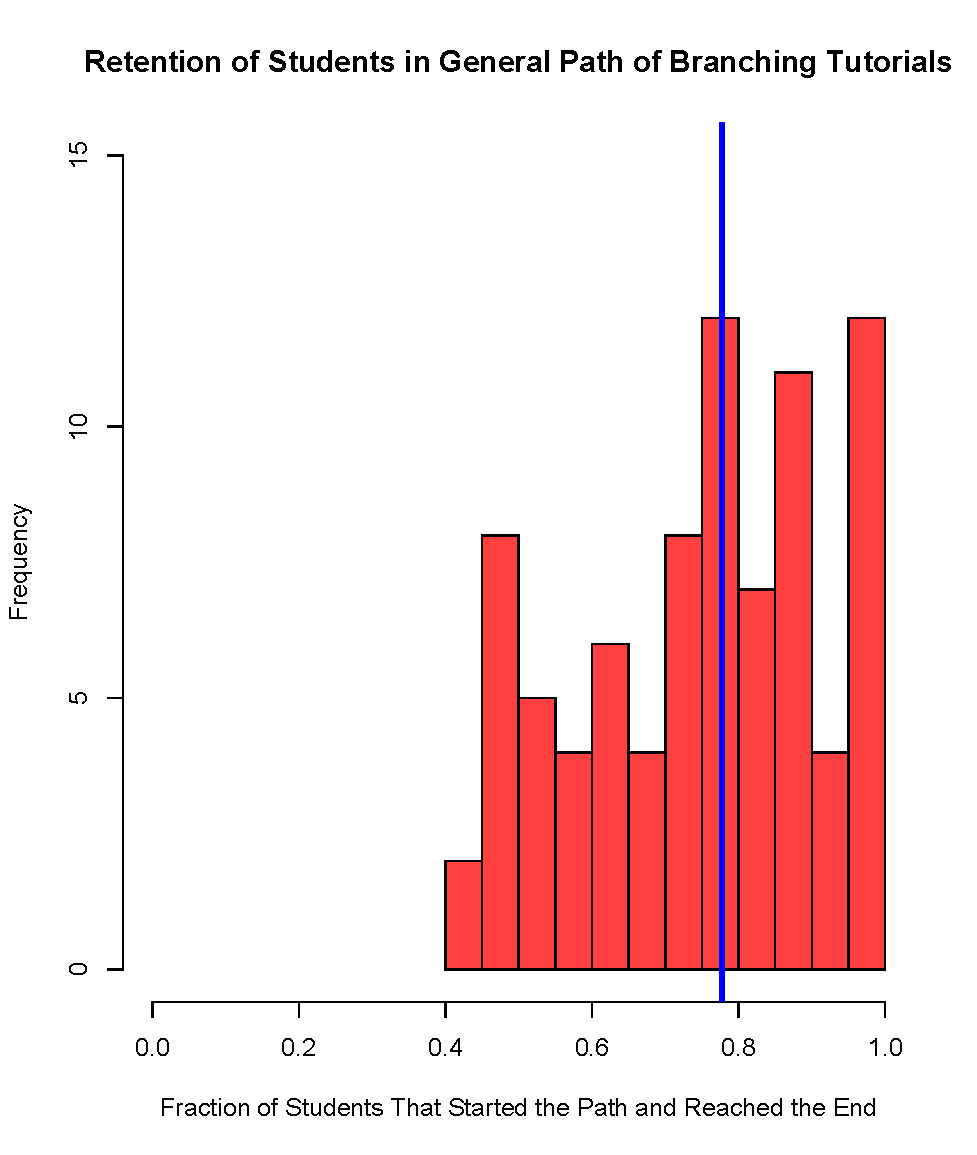
\includegraphics[width=0.46\textwidth]{img/retention_filtered.pdf}
		\caption{The figure on the left shows that, on average, 60\% of students who start a tutorial reach the final step. The figure on the right shows that, on average, 80\% of students who start a tutorial reach the second to the last step.}
		\label{fig:retention_examples}
	\end{figure}	
\end{frame}

\begin{frame}{Efficiency}
	\framesubtitle{Step Function}
	\begin{figure}
		\centering
		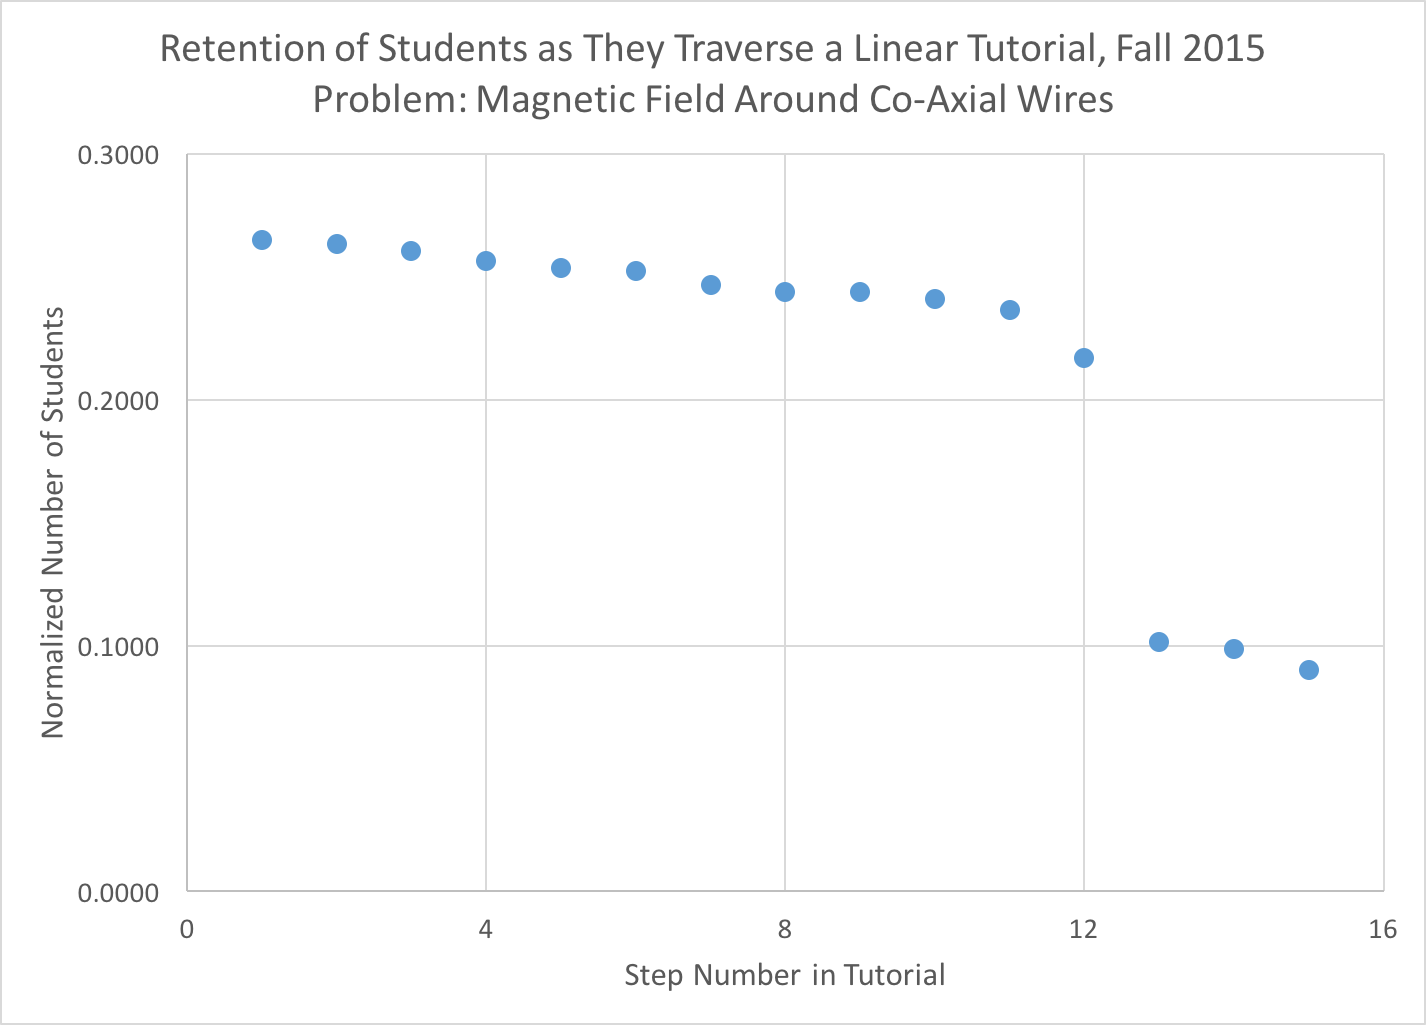
\includegraphics[width=0.6\textwidth]{img/step_function_1.png}
		\caption{Student retention as they pass over a tedious step in the tutorials.}
		\label{fig:step_function_examples}
	\end{figure}	
\end{frame}

\begin{frame}{Efficiency}
	\framesubtitle{Step Function}
	\begin{figure}
		\centering
		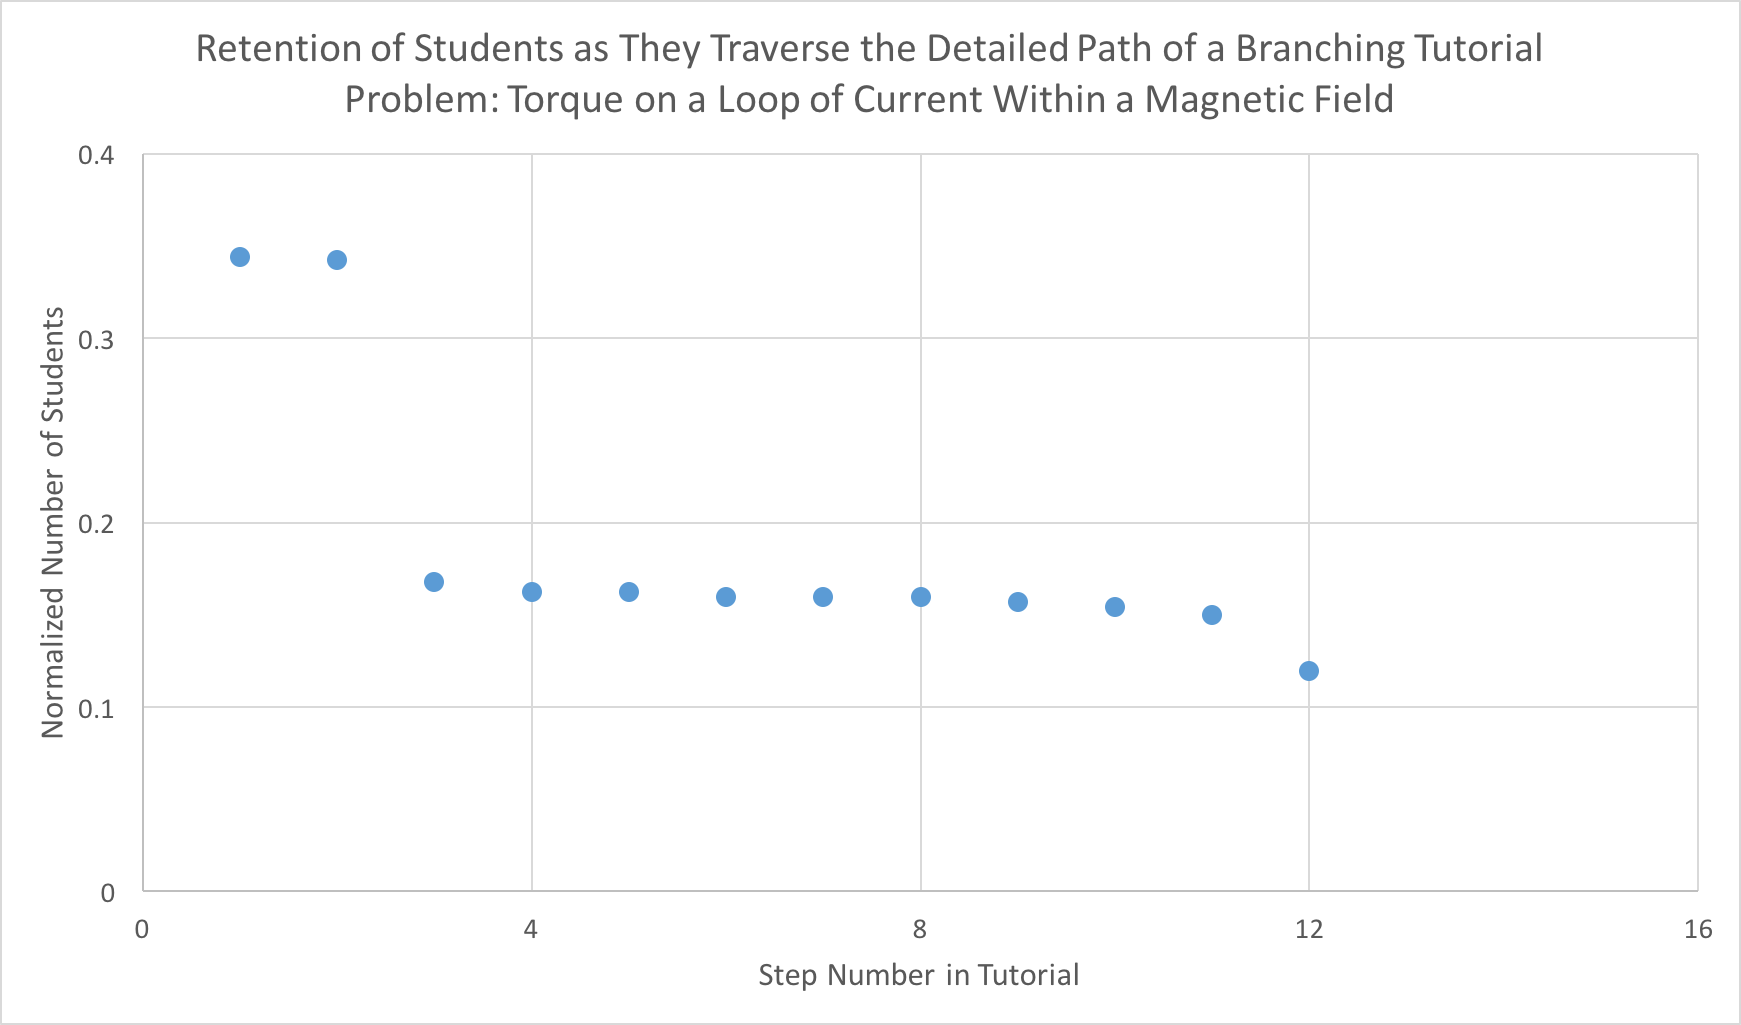
\includegraphics[width=0.6\textwidth]{img/step_function_2.png}
		\caption{A second example of student retention as they pass over a tedious step in the tutorials.}
		\label{fig:step_function_examples}
	\end{figure}	
\end{frame}

%%%%%%%%%%%%%%%%%%%%%%%%%%%%%%%%%%%%%%%%%%%%%%%%%%%%%%
%%%%%%%%%%%%%%%%%%%%%%%%%%%%%%%%%%%%%%%%%%%%%%%%%%%%%%

\section{\scshape Summary}

\subsection{Conclusions}

\begin{frame}{Summary of Results}
	\begin{itemize}
		\item We developed a number of tutorials that were paired with the homework problems.
		\item We saw small, but statistically significant gains for students who used the CITA tutorials.
		\item We studied how students used the tutorials within their work schedule.
		\begin{itemize}
			\item Students really liked Shallow CITA
			\item Students generally liked Immersive CITA
			\item Postscripts were generally never used
		\end{itemize}
	\end{itemize}
\end{frame}

\begin{frame}{Future Directions}
	\begin{itemize}
		\item Write Up Piazza Results
		\item Thematic Analysis of Online Homework Systems
		\item Cupcake Physics (My Own Little Education Site)
	\end{itemize}
\end{frame}

\begin{frame}{}
	\begin{center}
		{\large Questions?}
	\end{center}
\end{frame}

%%%%%%%%%%%%%%%%%%%%%%%%%%%%%%%%%%%%%%%%%%%%%%%%%%%%%%
%%%%%%%%%%%%%%%%%%%%%%%%%%%%%%%%%%%%%%%%%%%%%%%%%%%%%%

\appendix
\section{\scshape Backup Slides}

\subsection{Relationship Between P-Value and $R^2$}

\begin{frame}{Relationship Between P-Value and $R^2$}
	\begin{itemize}
		\item \textit{Large P, Large $R^2$:}\newline
		Data appears linear because there are few data points.
		\vspace{2mm}
		\item \textit{Large P, Small (or Negative) $R^2$:}\newline
		Data does not follow a linear model at all.
		\vspace{2mm}
		\item \textit{Small P, Large $R^2$:}\newline
		Data follows a linear model with a good fit.
		\vspace{2mm}
		\item \textit{Small P, Small $R^2$:}\newline
		Data follows a linear model, but the range of the data is large.
	\end{itemize}
\end{frame}

\subsection{Overall Grade vs. Number of Clicks for AP Physics Students}

\begin{frame}{Overall Grade vs. Number of Clicks}
	\framesubtitle{AP Physics Students}
	\begin{figure}
		\centering
		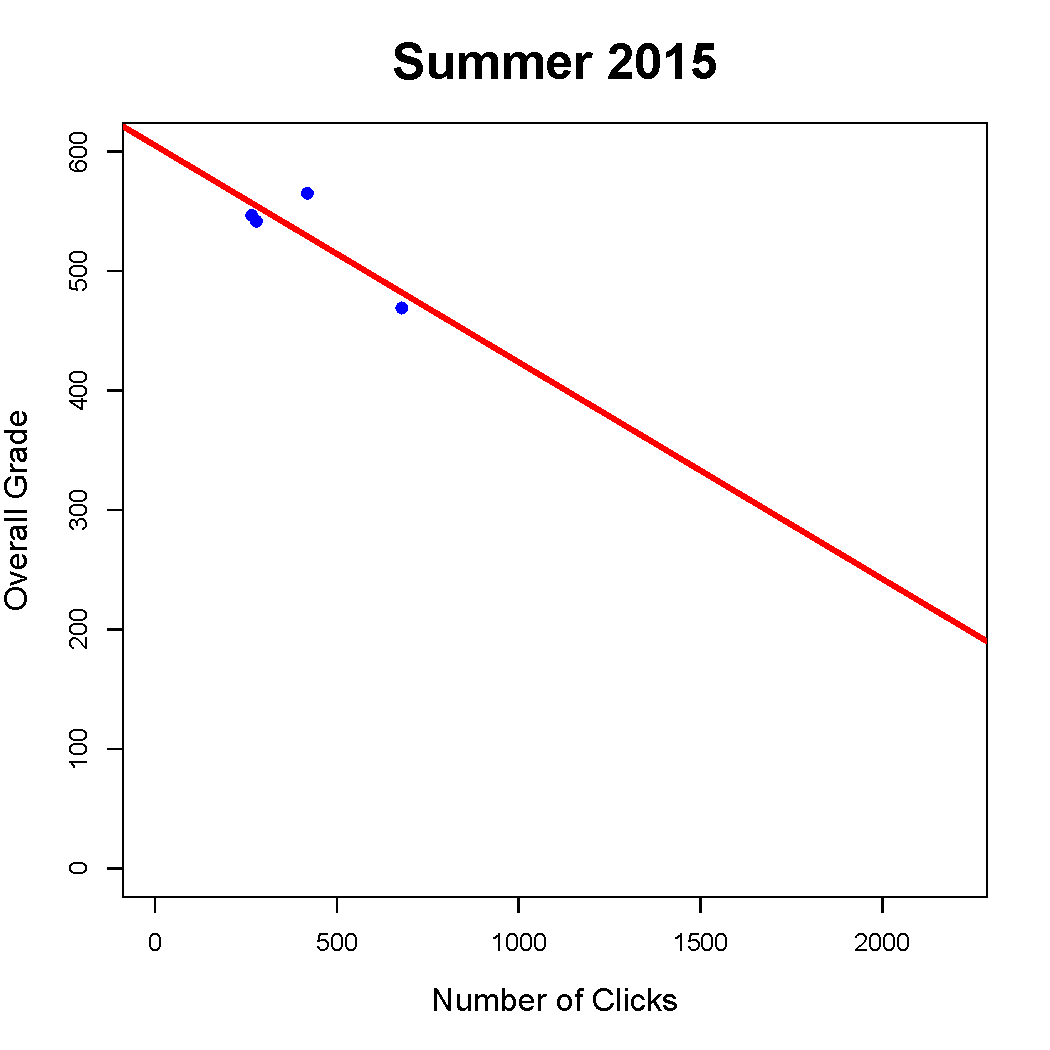
\includegraphics[width=0.33\textwidth]{img/overall_grade_vs_clicks_su15_ap_students.pdf}
		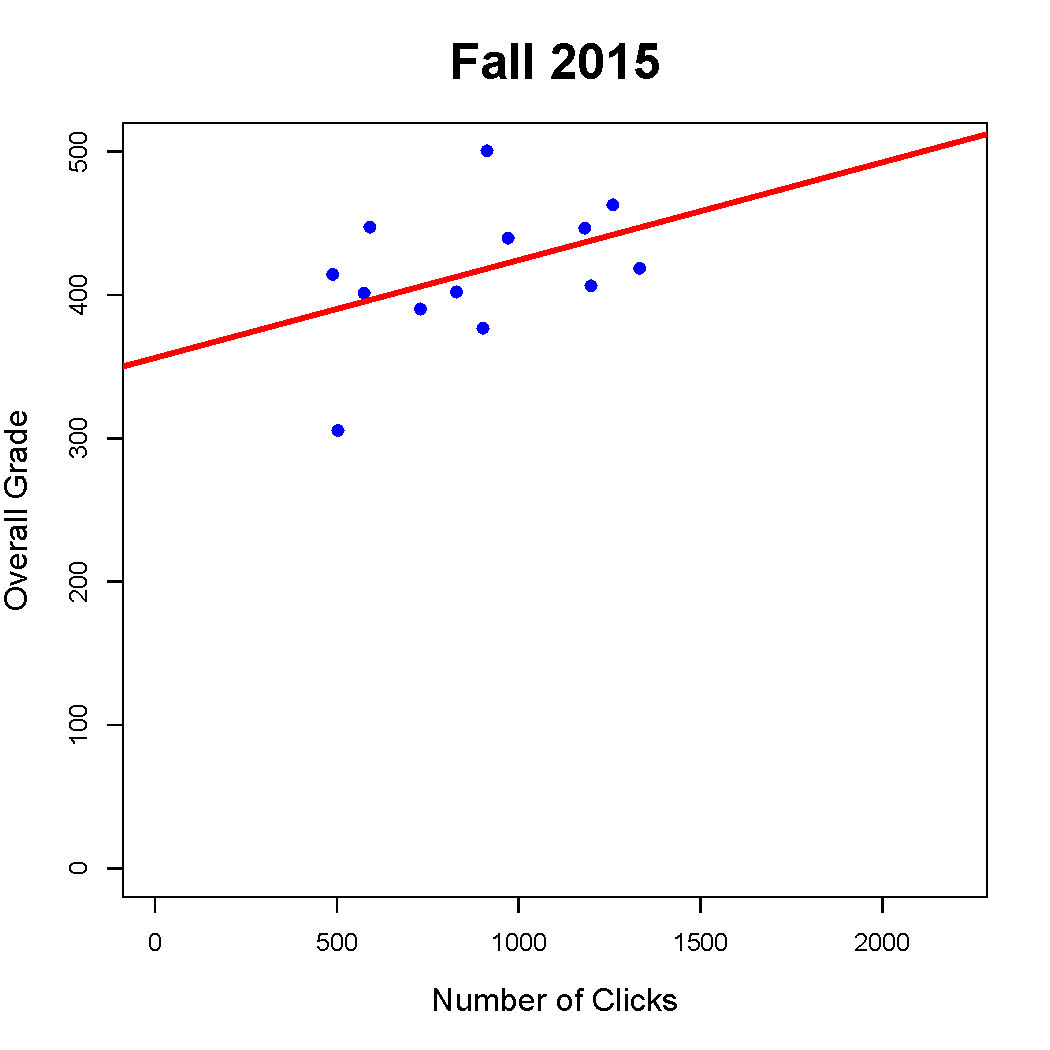
\includegraphics[width=0.33\textwidth]{img/overall_grade_vs_clicks_fa15_ap_students.pdf}
		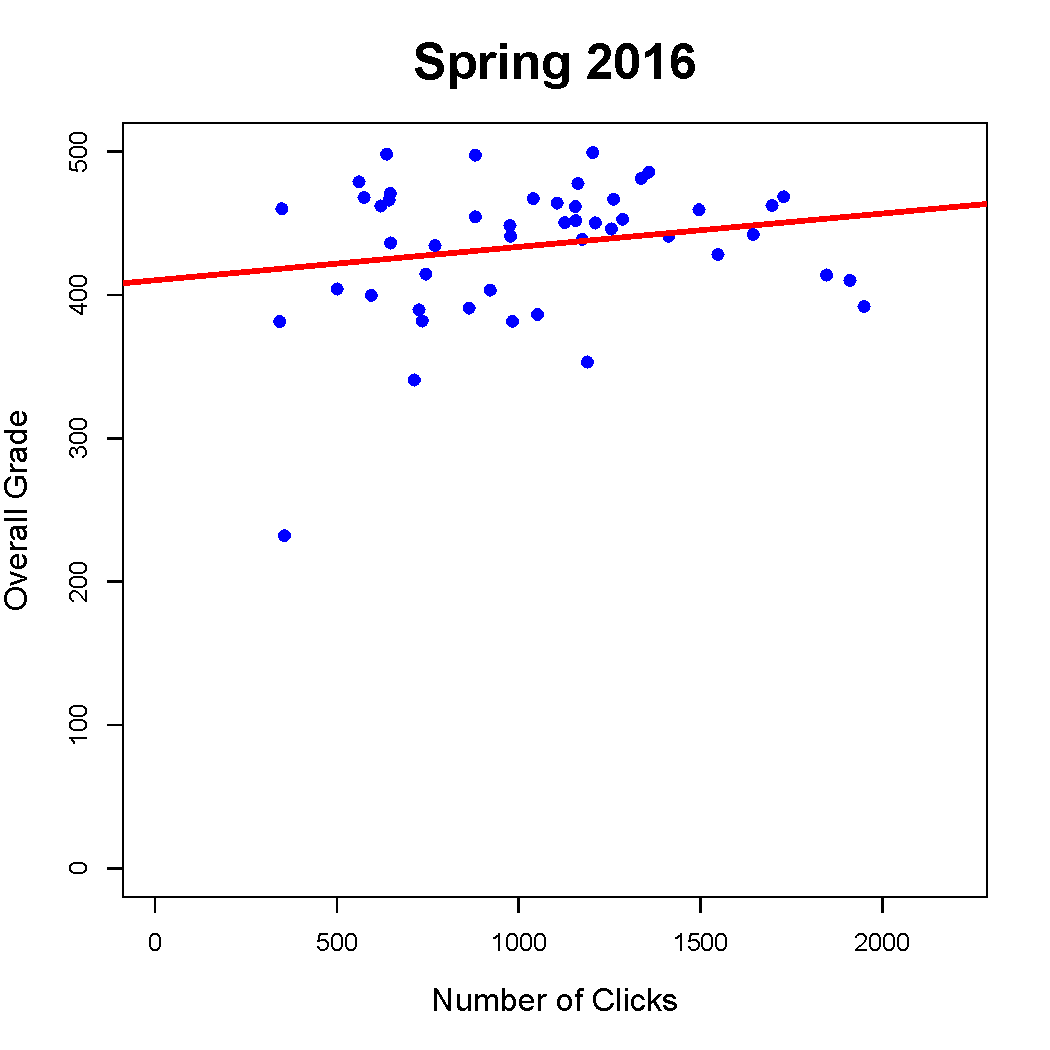
\includegraphics[width=0.33\textwidth]{img/overall_grade_vs_clicks_sp16_ap_students.pdf}
		\caption{In the summer and fall of 2015, a linear model did not fit the data due to the small sample sizes ($p = 0.177$ and $p = 0.146$, respectively). In the spring of 2016, a linear model did not fit the data due to the large range of Overall Grades ($p = 0.165$).}
		\label{fig:overall_grade_vs_clicks_ap_students}
	\end{figure}
\end{frame}

\subsection{Individual Grade Components}

\begin{frame}{Source of Gains}
	A few notes...
	\begin{itemize}
		\item Out of the five types of graded components of PHYS 24100, three of them showed a prominent ceiling effect.
		\item Even in cases where the linear model applied, the effect sizes were generally small ($R^2 < 0.10$).
		\item It is difficult to compare the non-normalized linear models for the Overall Grades and the grade components. Thus, I will scale the slope from the linear models by their maximum y-value in order to normalize them.
	\end{itemize}
	\vspace{3mm}
	\begin{equation}
		m_{max} = \frac{0.086 \hspace{1mm} points/click}{500 \hspace{1mm}  points} = 1.7 \times 10^{-4}
	\end{equation}
	\begin{equation}
		m_{min} = \frac{0.018  \hspace{1mm} points/click}{500 \hspace{1mm}  points} = 3.6 \times 10^{-5}
	\end{equation}
\end{frame}

\begin{frame}{Overall Homework Grade}
	\framesubtitle{Cut By PHYS 17200 Grade}
	\begin{figure}
		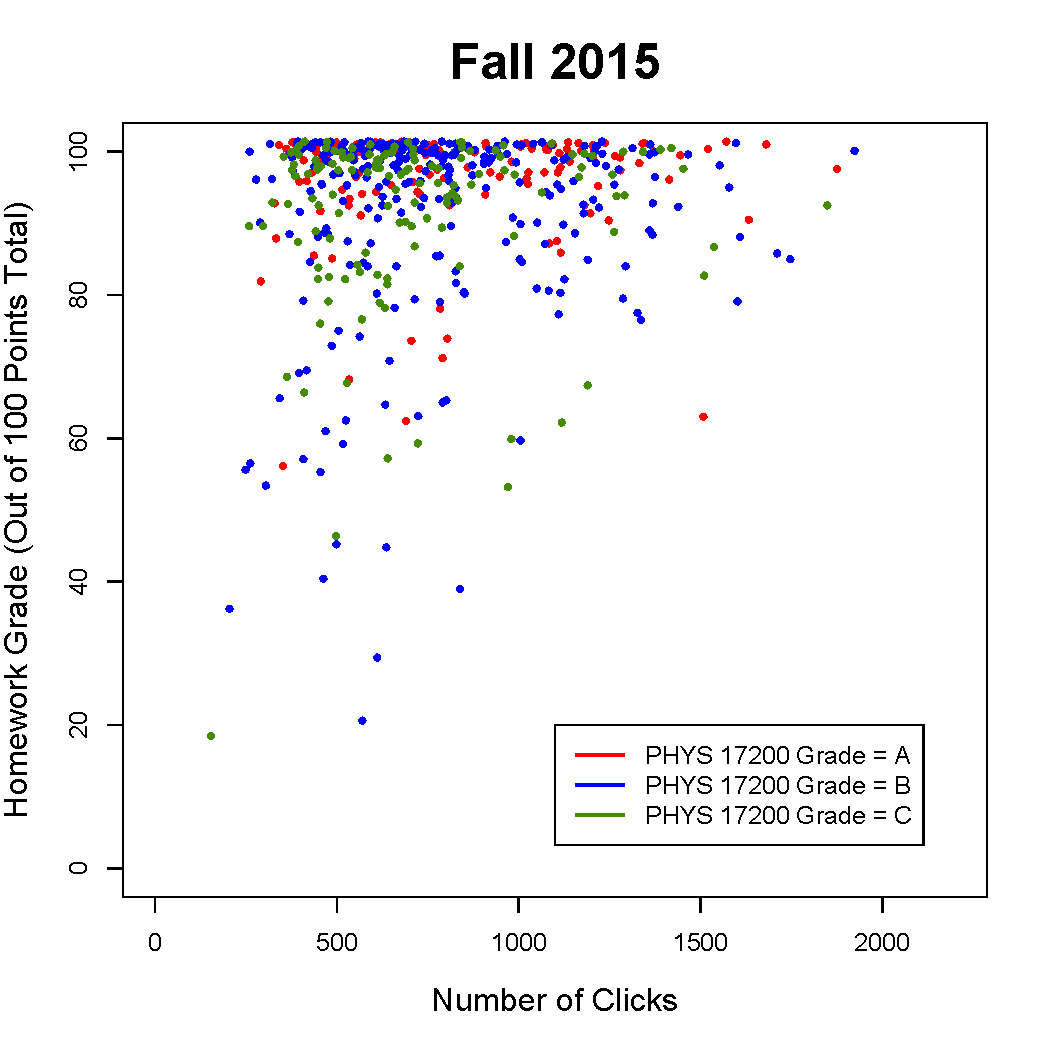
\includegraphics[width=0.5\textwidth]{img/homework_fa15_172.pdf}
		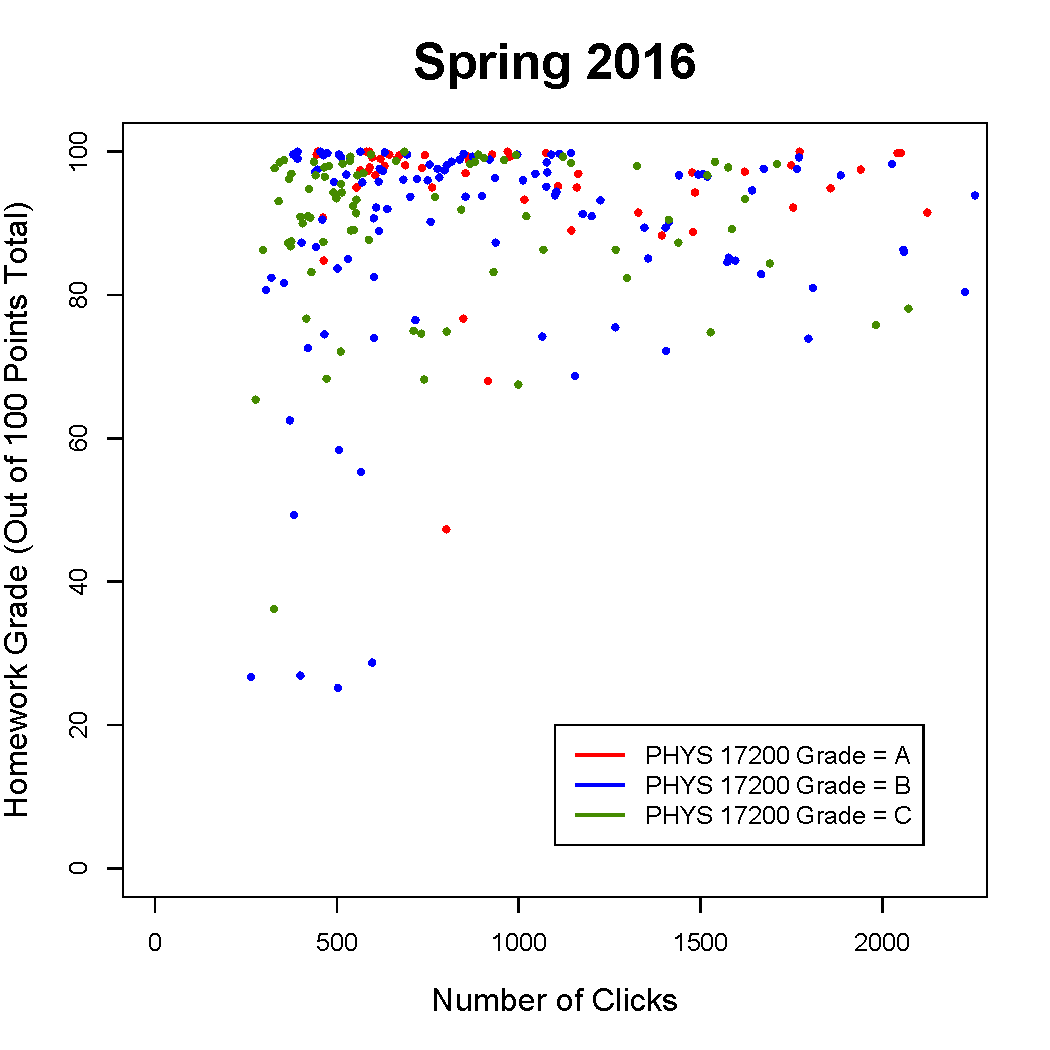
\includegraphics[width=0.5\textwidth]{img/homework_sp16_172.pdf}
	\end{figure}
\end{frame}

\begin{frame}{Overall Recitation Grade}
	\framesubtitle{Cut By PHYS 17200 Grade}
	\begin{figure}
		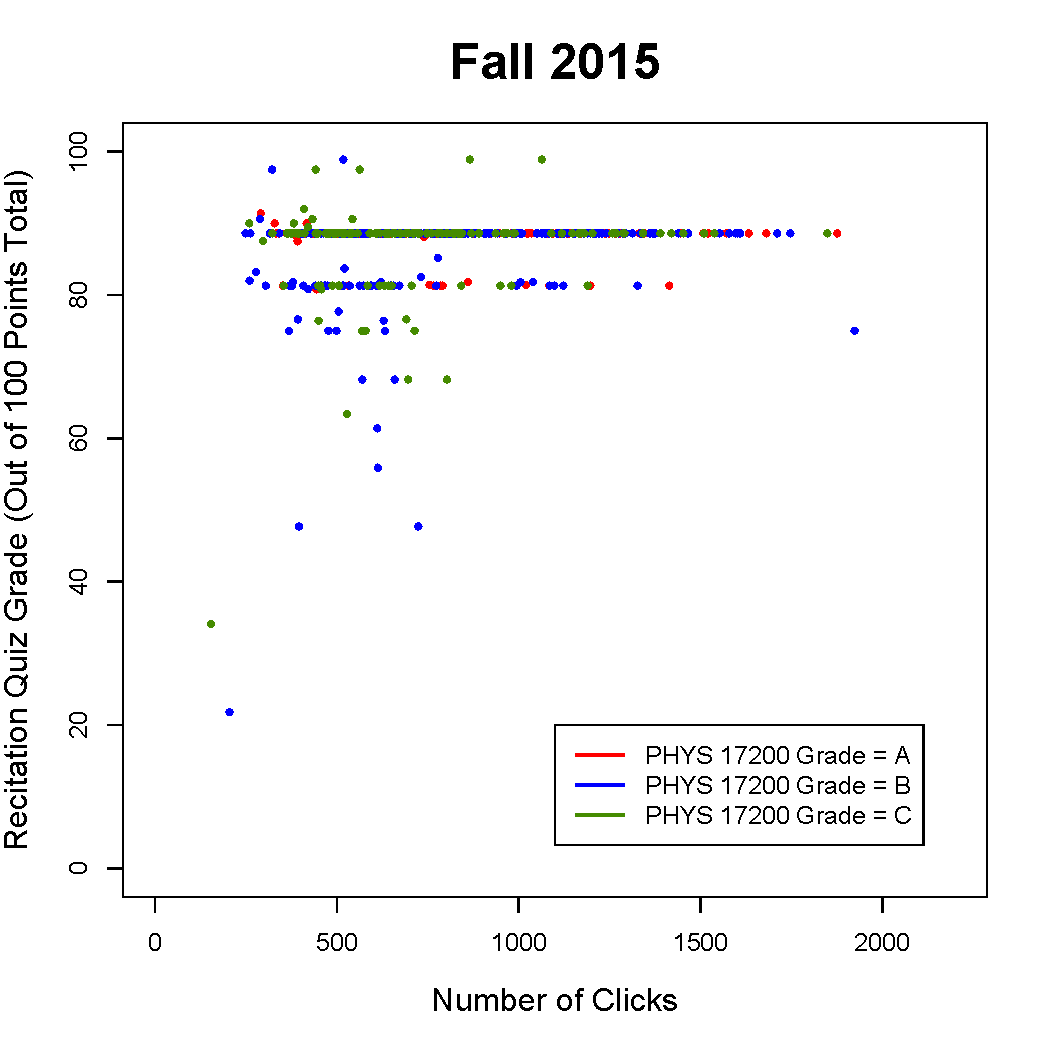
\includegraphics[width=0.5\textwidth]{img/recitation_fa15_172.pdf}
		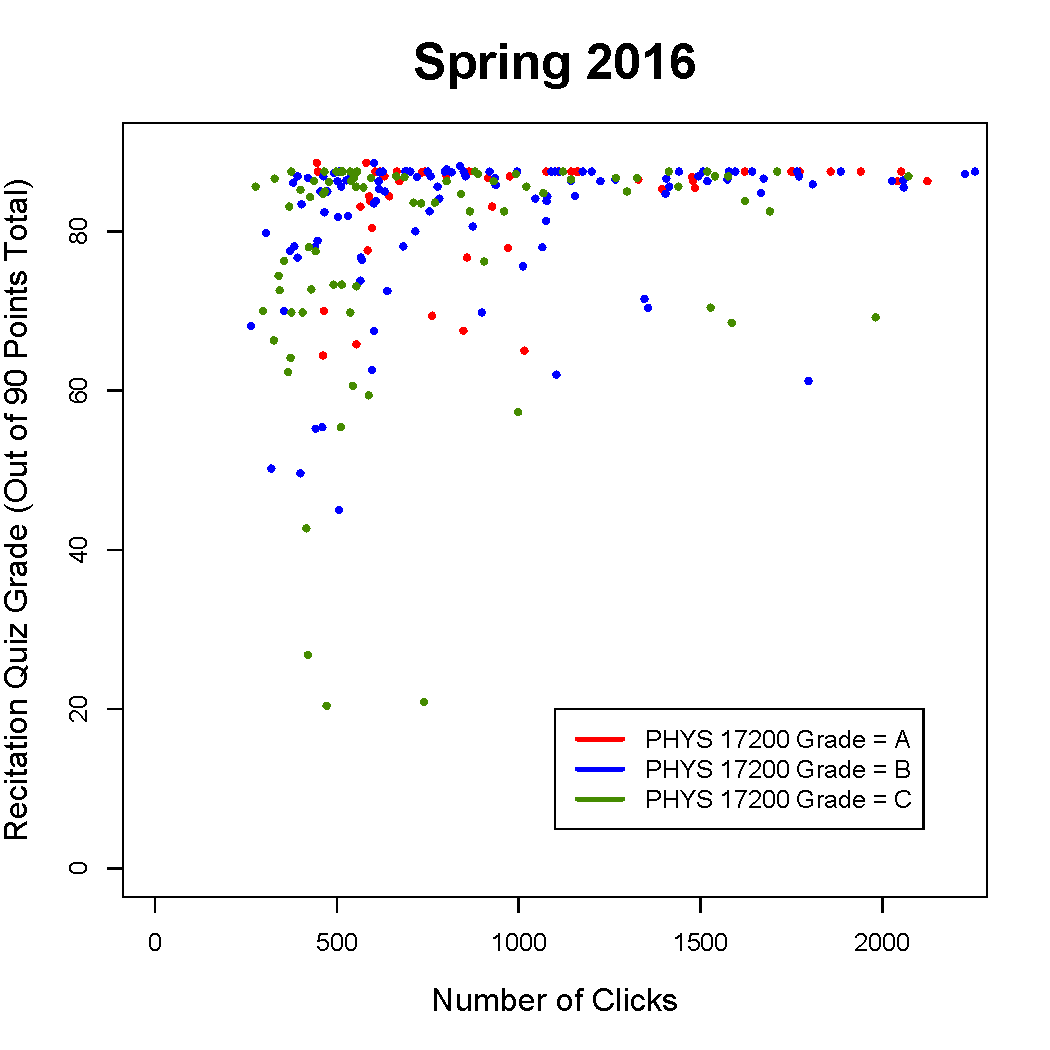
\includegraphics[width=0.5\textwidth]{img/recitation_sp16_172.pdf}
	\end{figure}
\end{frame}

\begin{frame}{Overall Lecture Quiz Grade}
	\framesubtitle{Cut By PHYS 17200 Grade}
	\begin{figure}
		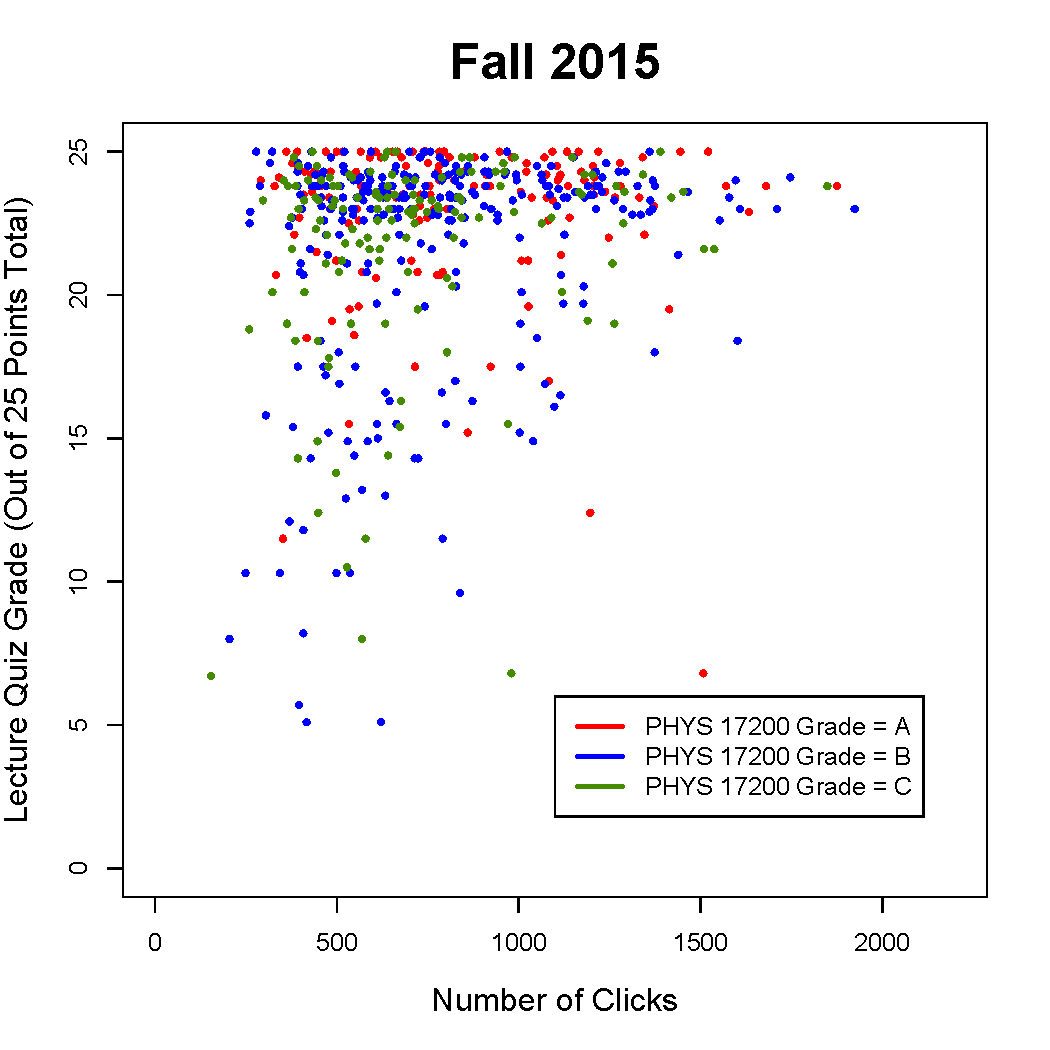
\includegraphics[width=0.5\textwidth]{img/lecture_fa15_172.pdf}
		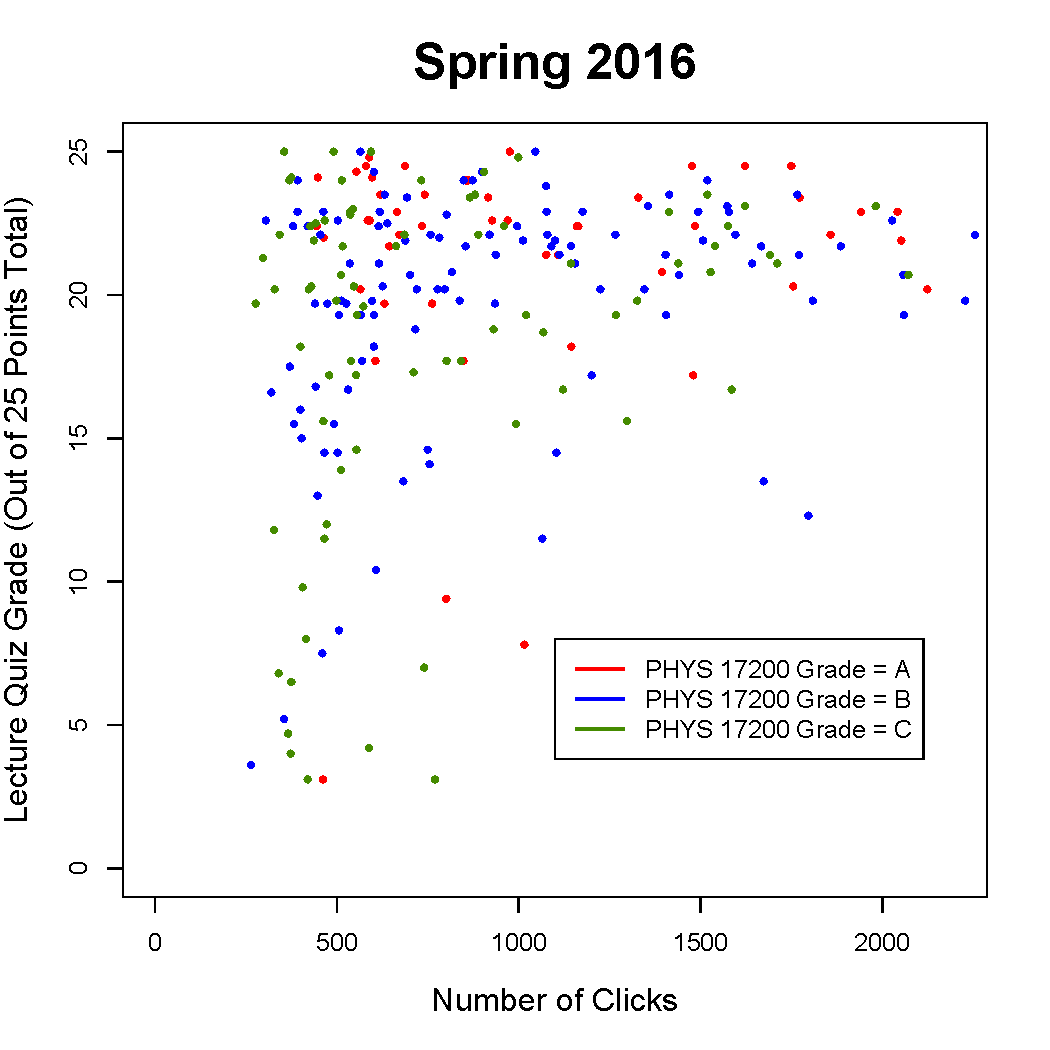
\includegraphics[width=0.5\textwidth]{img/lecture_sp16_172.pdf}
	\end{figure}
\end{frame}

\begin{frame}{Midterm Exams}
	\framesubtitle{Cut By PHYS 17200 Grade}
	\begin{figure}
		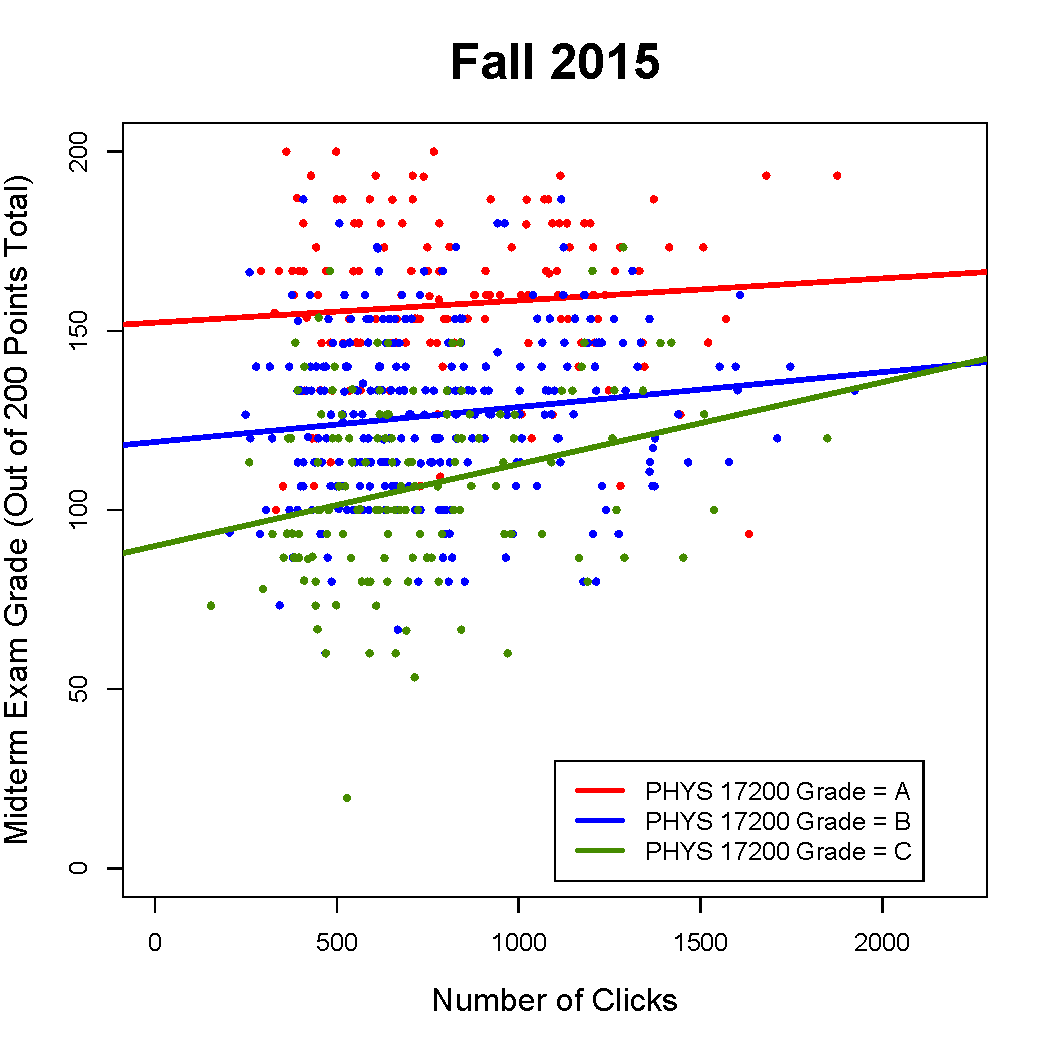
\includegraphics[width=0.44\textwidth]{img/exam_fa15_172.pdf}
		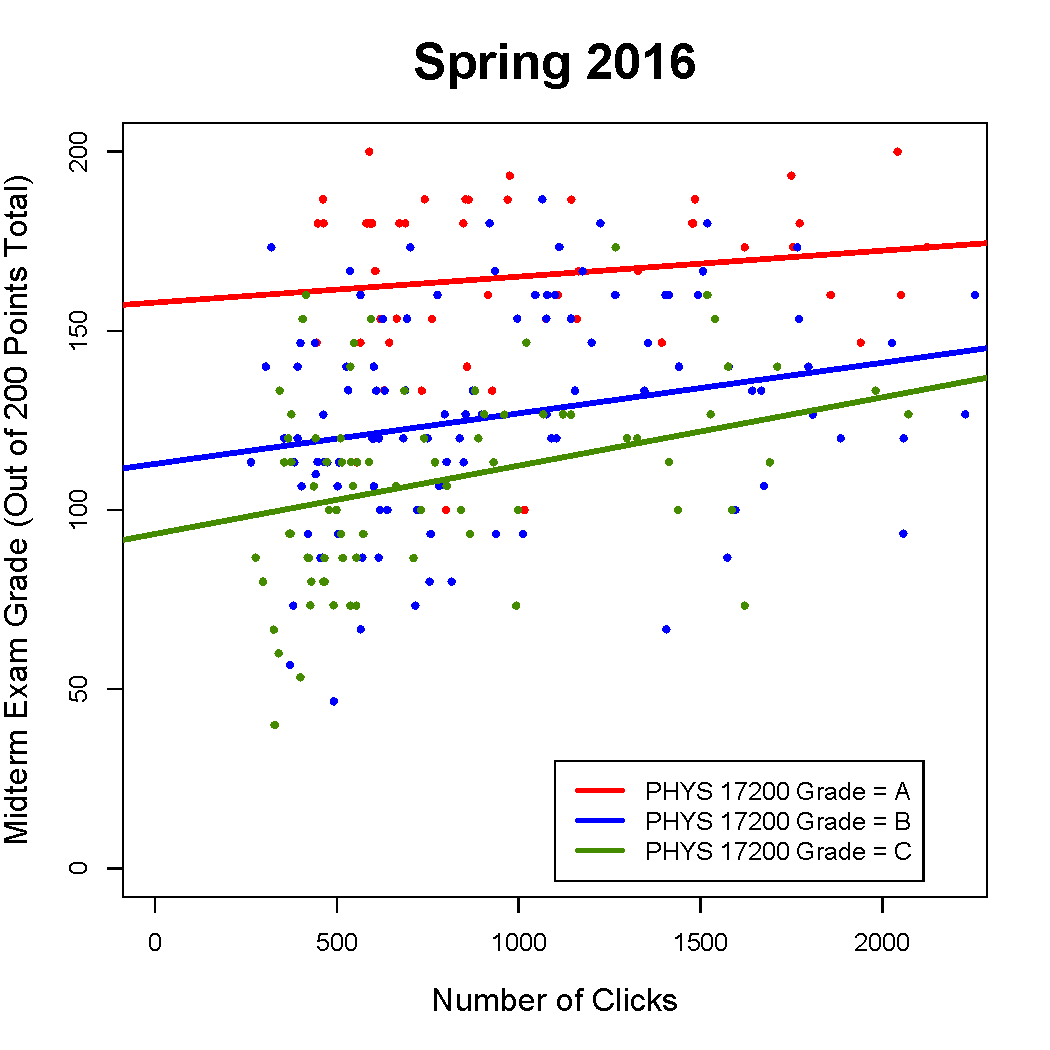
\includegraphics[width=0.44\textwidth]{img/exam_sp16_172.pdf}
	\end{figure}
	These linear models did have statistically significant fits ($ p < 0.05$), and the normalized slopes were in the range of $m = 0.01 / 200 = 5.0 \times 10^{-5}$ to $m = 0.02 / 200 = 1.0 \times 10^{-4}$.
\end{frame}

\begin{frame}{Final Exam}
	\framesubtitle{Cut By PHYS 17200 Grade}
	\begin{figure}
		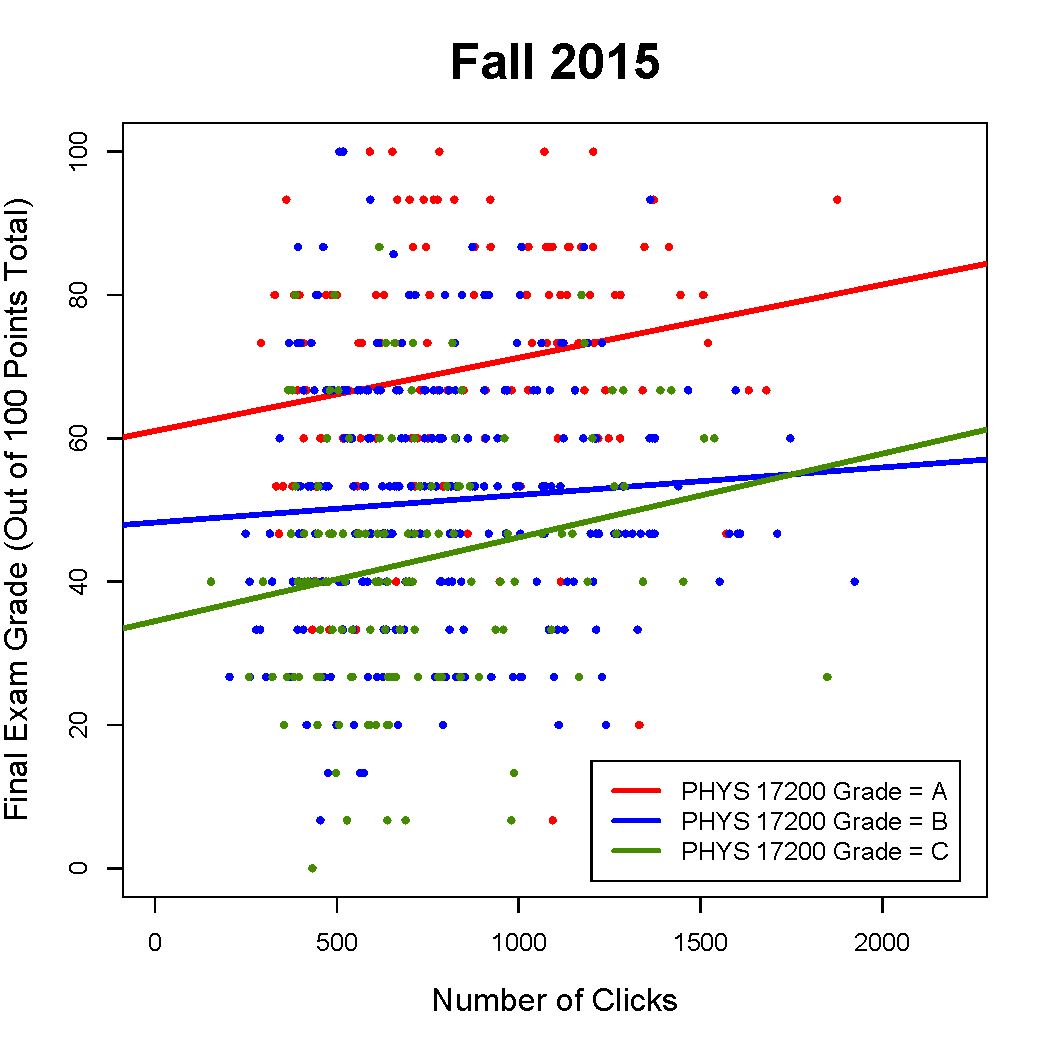
\includegraphics[width=0.44\textwidth]{img/final_fa15_172.pdf}
		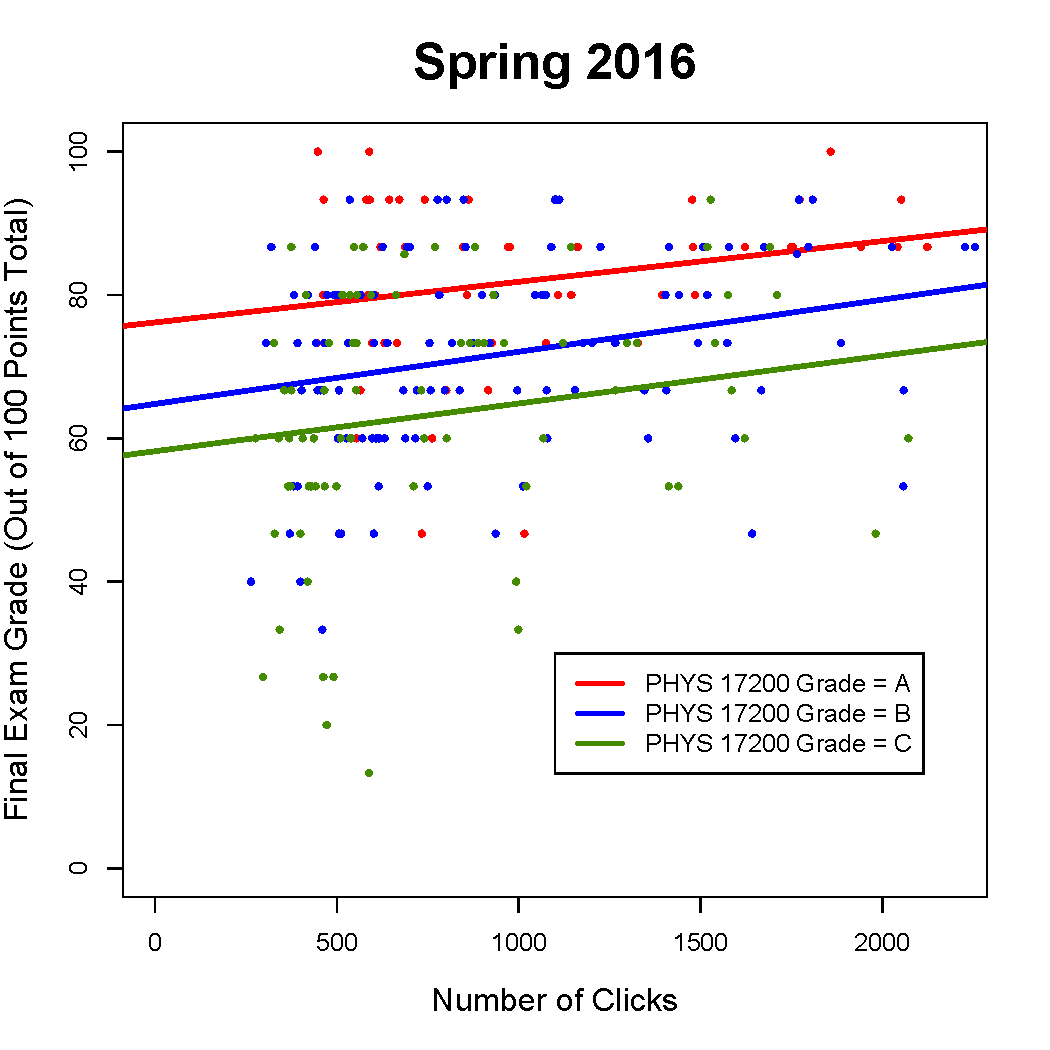
\includegraphics[width=0.44\textwidth]{img/final_sp16_172.pdf}
	\end{figure}
	These linear models did have statistically significant fits ($ p < 0.05$), and the normalized slopes were in the range of $m = 0.007 / 100 = 7.0 \times 10^{-5}$ to $m = 0.01 / 100 = 1.0 \times 10^{-4}$.
\end{frame}

%%%%%%%%%%%%%%%%%%%%%%%%%%%%%%%%%%%%%%%%%%%%%%%%%%%%%%
%%%%%%%%%%%%%%%%%%%%%%%%%%%%%%%%%%%%%%%%%%%%%%%%%%%%%%

\end{document}
